\documentclass[11pt,letterpaper]{book}
\usepackage[utf8]{inputenc}
\usepackage[left=1in,right=1in,top=1in,bottom=1in]{geometry}
\usepackage{amsmath,amsthm,amsfonts,amssymb,amscd}
\usepackage{mathtools,mathrsfs}
\usepackage{lastpage}
\usepackage{enumerate}
\usepackage{graphicx}
\usepackage{wrapfig}

\usepackage[style=alphabetic]{biblatex}
\addbibresource{citation.bib}

\usepackage{hyperref}
\hypersetup{
    colorlinks=true,
    linkcolor=blue,    
    urlcolor=blue,
    citecolor=blue
}
% \usepackage{cleveref}

\setlength{\parindent}{0.0in}
\setlength{\parskip}{0.1in}

\newtheorem*{theorem}{Theorem}
\newtheorem*{lemma}{Lemma}
\newtheorem*{corollary}{Corollary}
\newtheorem*{remark}{Remark}
\theoremstyle{definition}
\newtheorem*{definition}{Definition}

%%%%%%%%%%%%%%%%%%
\newcommand{\de}{\mathrm{d}}
\newcommand{\pe}{\partial}

\newcommand{\dsp}{\displaystyle}

\newcommand{\norm}[1]{\left\Vert #1 \right\Vert}

\newcommand{\ve}[1]{\boldsymbol{#1}}

\newcommand{\thus}{\Rightarrow \quad }
\newcommand{\fff}{\iff\quad}

\newcommand{\re}{\text{Re}}
\newcommand{\im}{\text{Im}}

\newcommand{\APE}{\text{APE}}
\newcommand{\KE}{\text{KE}}

\newcommand{\hot}{\text{h.o.t.}}
\newcommand{\inner}[2]{\left\langle #1,#2\right\rangle}


\newcommand{\ssp}{\left.\qquad\right.}
%%%%%%%%%%%%%%%%%%%

%\titleformat{\subsection}[runin]
%        {\normalfont\bfseries}
%        {(\arabic{section}.\alph{subsection})}% the label and number
%        {0.5em}% space between label/number and subsection title
%        {}% formatting commands applied just to subsection title
%        []% punctuation or other commands following subsection title

\begin{document}
\renewcommand\thesection{\arabic{section}.}
\renewcommand\thesubsection{(\arabic{section}.\alph{subsection})}

\setcounter{tocdepth}{1}
\tableofcontents

\chapter{READ ME}
Source code is available at \url{https://github.com/Empyreal092/GFD-Written-Solutions}.

This document contains the erreta and some solutions to the GFD Written Exam at NYU Courant. The exams are in the ``Problem\_packages" folder and is available by request from the department.

Read Chapter \ref{chap:erreta} - Erreta before doing the problems might save you some time and pain. It contains the (possible) errors of the problems. 

The rest of the documents are (extended or terse) answers for some the problems in the written exam.

There most definitely will be errors so be mindful when you read the solutions. When you find any, please let me know at \url{ryan_sjdu@nyu.edu}. 

If you have also typed up solutions, I am happy to include yours in this document (with acknowledgement), or let my solutions be a part of your document. The goal is for there to be close to full solutions to all problems. 

I had help from Professor Olivier Pauluis, who taught me GFD, the solutions produced by past GFD students, and my 2020 peers.


\chapter{Erreta}\label{chap:erreta}
\section{Jan 2010, Problem 2}
The proposed streamfunction in the question, when plugged into the SWQG in P1, will not produce the Rayleigh equation we are asked to show. Because $U$ is not constant, $(yU)'$ has to use the product rule and produce a big mess. Use $\psi_y$ = $\psi'_y-U$ would lead to the right/intended Rayleigh equation (of course $U$ is not in the unit of velocity but unit of streamfunction).

\section{Jan 2010, Problem 3}
In part (b) also assume adiabatic.

\section{Sep 2010, Problem 4}
In part (b) study $t\to \infty$ instead.

\section{Jan 2012, Problem 3}
Aug 2017, Problem 3 is the same and is a bit more friendly. See erreta \ref{err:aug_2017_3}. 

\section{Jan 2014, Problem 3}
In part (e) the 2 in the second equation should not be there.

\section{Jan 2015, Problem 3}\label{err:jan_2015_3}
Part (c), the group velocity is positive thus the should wave moves east.

\section{Aug 2016, Problem 2}
$u$ is the azimuthal velocity and $v$ is the radial. The matrial derivative is
\begin{align*}
    \frac{D}{Dt} = \pe_t+\frac{1}{r}u\pe_\theta+v\pe_r
\end{align*}
(cf. Jan 2015 Problem 1).

\section{Aug 2017, Problem 3}\label{err:aug_2017_3}
For part (d), try $\psi = \sqrt{\overline{u}-c}\;\phi$ instead.

\chapter{Aug 2002}
\section{Physics of Fluids - Stokes' Law}
$F\sim R^3$, thus $V\sim R^2$, very small.

\chapter{Aug 2003}
\section{Ekman Layers}
See Vallis.

\section{Dry Atmospheric Thermodynamics}
\subsection{}
Adiabatic, $\de s = 0$.

\subsection{}
We have
\begin{align*}
    c_p\de T = T\de S+\alpha\de p = T\de S+\frac{RT}{p}\de p
\end{align*}
then we have
\begin{align*}
    &\de s = c_p\de\ln T-R\de\ln p = c_p\de\ln\theta\\
    \thus &s = c_p\ln T-R\ln p+C
\end{align*}

\subsection{}
Standard, result:
\begin{align*}
    \frac{\de T}{\de z} = -gc_p
\end{align*}
We know that
\begin{align*}
    N^2 = \frac{g}{\theta}\frac{\de\theta}{\de z}
\end{align*}
therefore stable regime ($N^2>0$) correspond to increasing $\theta$ with height.

\subsection{}
Follow from
\begin{align*}
    \left(\frac{\pe p}{\pe x}\right)_\theta = \left(\frac{\pe p}{\pe x}\right)_z+\left(\frac{\pe p}{\pe z}\right)_x\left(\frac{\pe z}{\pe x}\right)_\theta
\end{align*}
which is justified by drawing a picture.

\subsection{}
We use the formula above, and
\begin{align*}
    \alpha\left(\frac{\pe p}{\pe x}\right)_\theta = c_p\left(\frac{\pe T}{\pe x}\right)_\theta
\end{align*}
because of adiabaticity. 


\chapter{Sep 2004}
\section{Thermodynamics}
\subsection{}
Standard derivation, we have
\begin{align*}
    \theta = T\left(\frac{p_R}{p}\right)^{R/c_p}
\end{align*}

Follow from the formula from the next part, const $\theta$ gives constant $\eta$.

\subsection{}
Standard derivation gives:
\begin{align*}
    \de s = c_p\de\ln T-R\de\ln p
\end{align*}
Then
\begin{align*}
    c_p\de\ln\theta = c_p\frac{1}{\theta}\de\theta = c_p\de\ln T-R\de\ln p
\end{align*}
follows after some calculation.

\subsection{}
We have
\begin{align*}
    &\frac{\de Q}{\de t} = T\frac{\de \eta}{\de t}\\
    &\frac{\de \eta}{\de t} = \frac{1}{T}\frac{\de Q}{\de t}
\end{align*}
but also
\begin{align*}
    \frac{\de \eta}{\de t} = \frac{c_p}{\theta}\frac{\de\theta}{\de t}.
\end{align*}
Therefore
\begin{align*}
    \frac{\de\theta}{\de t} &= \frac{\theta}{c_p T}\frac{\de Q}{\de t}\\
    &= \frac{1}{c_p}\left(\frac{p_R}{p}\right)^{R/c_p}\frac{\de Q}{\de t}.
\end{align*}

\subsection{}
We have
\begin{align*}
    \frac{\de\rho}{\de t} &= \frac{\pe\rho}{\pe p}\frac{\de p}{\de t}+\frac{\pe\rho}{\pe q}\frac{\de q}{\de t}+\frac{\pe\rho}{\pe \theta}\frac{\de p\theta}{\de t}\\
    &= \frac{\pe\rho}{\pe p}\frac{\de p}{\de t}+\frac{\pe\rho}{\pe q}\frac{\de q}{\de t}+\frac{\pe\rho}{\pe \theta}\frac{1}{c_p}\left(\frac{p_R}{p}\right)^{R/c_p}\frac{\de Q}{\de t}.
\end{align*}


\chapter{Jan 2005}
\section{Turbulence}

\section{Ray Tracing}

% \chapter{Jan 2006}

\chapter{Jan 2008}
\section{Baroclinic instability}
ok

% \chapter{Aug 2008}

\chapter{Jan 2010}
\section{Rossby Wave}
Same as Aug 2012 Problem \ref{prob:Aug_2012_2}.
\subsection{}

\subsection{}\label{prob:jan_2010_1_b}

\subsection{}
\begin{align*}
&\frac{kU(k^2+\ell^2)-k\beta}{k^2+\ell^2+F} = 0\\
\thus &U(k^2+\ell^2) = \beta\\
\thus &\lambda = \frac{2\pi}{\sqrt{{\beta}/{U}}}.
\end{align*}
We have the dimensional value for the atmosphere $\beta \sim 10^{-11}$ and $U\sim 10$ m/s. Then
\begin{align*}
\lambda\sim 10^6\text{ m}\sim 10^3\text{ km}.
\end{align*}
The wavelength of the meander of subpolar jet stream.

\section{Barotropic Instability}
The proposed streamfunction in the question, when plugged into the SWQG in P1, will not produce the Rayleigh equation we are asked to show. Because U is not constant, $(yU)'$ has to use the product rule and produce a big mess. Use $\psi_y = \psi'_y-U$ would lead to the right Rayleigh equation (of course $U$ here is not in the unit of velocity, but in unit of streamfunction).

Necessary condition:
\begin{align*}
\beta+FU-U_{yy}
\end{align*}
must change sign in the domain. $FU$ is the PV gradient due to finite deformation radius (cf. \ref{prob:jan_2010_1_b}). 

\section{Ideal Gas Thermodynamics}\label{Jan_2010_Prob3}
\subsection{}
We have
\begin{align*}
\de Q = \de I+p\de \alpha.
\end{align*}
And for ideal gas: 
\begin{align*}
I &= c_v T\\
p\alpha &= RT.
\end{align*}
Then
\begin{align*}
\de Q &= c_v\de T+ \de(RT)-\alpha\de p\\
&= (c_v+R)\de T-\alpha\de p.
\end{align*}
Finally we have
$$c_p = c_v+R.$$

\subsection{}\label{jan_2010_3_2}
Assume adiabaticity, $\de Q = 0$. Then
\begin{align*}
&c_p\de T = \alpha\de p\\
\thus &c_p\frac{\de T}{\de z} = \alpha\frac{\de p}{\de z}.
\end{align*}
From hydrostacity we have
\begin{align*}
\frac{\de p}{\de z} = -\rho g
\end{align*}
Thus
\begin{align*}
\frac{\de T}{\de z} = \frac{-g}{c_p}.
\end{align*}
Integrating this we obtain
\begin{align*}
T(z) = T_s-\Gamma_dz
\end{align*}
where $\Gamma_d = g/c_p$.

\subsection{}
Similar to \ref{jan_2010_3_2}, we have
\begin{align*}
c_p\frac{\de T}{\de z} = \alpha\frac{\de p}{\de z}.
\end{align*}
Replace $T$ with the result of \ref{jan_2010_3_2} and $\alpha = RT/p$, we have
\begin{align*}
&-c_p\Gamma_d = -g = \frac{RT}{p} \frac{\de p}{\de z}\\
&\frac{1}{p}\frac{\de p}{\de z} = \frac{-g}{RT} = \frac{-g}{R}\frac{1}{T_s-\Gamma_dz}\\
&\frac{\de}{\de z}\ln(p) = \frac{-c_p}{R}\frac{\de}{\de z}(T_s-\Gamma_d z)
\end{align*}
This gives
\begin{align*}
p(z) = p_s\left(\frac{T_s-\Gamma_d z}{T_s}\right)^{c_p/R}.
\end{align*}

\section{Energy Flux of Sahara Air}\label{Jan_2010_4}
Similar to Jan 2017 Problem \ref{prob:jan_2017_1}.

We have
\begin{align*}
\frac{\de H}{\de t} &= \rho\frac{\de Q}{\de t} \\
&= \rho\left(c_p\frac{\de T}{\de t}-\alpha\frac{\de p}{\de t}\right)\\
&= \rho\left(c_p\frac{\de T}{\de z}w-\alpha\frac{\de p}{\de z}w\right)\\
&= \rho\left(c_p\Gamma_e w+gw\right)
\end{align*}
where in the last step we used the hydrostatic balance. Then 
\begin{align*}
    J = Z\frac{\de H}{\de t}
\end{align*}
is the flux to space per area ($Z$ is the height of atmosphere).

\section{Two-Layer Shallow Water}
We have the shallow water equations:
\begin{align*}
&\frac{\pe \ve u_1}{\pe t}+(\ve u_1\cdot\nabla)\ve u_1+\ve f\times \ve u_1 = -\frac{1}{\rho_1}\nabla p_1 ;\\
&\frac{\pe \ve u_2}{\pe t}+(\ve u_2\cdot\nabla)\ve u_2+\ve f\times \ve u_2 = -\frac{1}{\rho_2}\nabla p_2 .
\end{align*}
where
\begin{align*}
p_1 &= \rho_1g(\eta_0-z);\\
p_2 &= \rho_1 g (\eta_0-\eta_1)+\rho_2 g (\eta_1-z)\\
&= \rho_1 g (\eta_0-z)-\rho_1 g (\eta_1-z)+\rho_2 g (\eta_1-z)\\
&= \rho_1[ g (\eta_0-z)+g' (\eta_1-z)].
\end{align*}
where
\begin{align*}
g' = \frac{\rho_2-\rho_1}{\rho_1}.
\end{align*}
Thus
\begin{align*}
\nabla p_1 &= \rho_1g\nabla \eta_0;\\
\nabla p_2 &= \rho_1[ g \nabla \eta_0+g' \nabla \eta_1].
\end{align*}
Then we have the equation
\begin{align}
&\frac{\pe \ve u_1}{\pe t}+(\ve u_1\cdot\nabla)\ve u_1+\ve f\times \ve u_1 = -g\nabla \eta_0 ;\label{eq:jan_2010_1}\\
&\frac{\pe \ve u_2}{\pe t}+(\ve u_2\cdot\nabla)\ve u_2+\ve f\times \ve u_2 = -\frac{\rho_1}{\rho_2}[ g \nabla \eta_0+g' \nabla \eta_1] .\label{eq:jan_2010_2}
\end{align}
We also have the mass conservation equation for the both layers:
\begin{align}
&\frac{\pe h_1}{\pe t}+\nabla\cdot(\ve u_1 h_1) = 0;\label{eq:jan_2010_3}\\
&\frac{\pe h_2}{\pe t}+\nabla\cdot(\ve u_2 h_2) = 0.\label{eq:jan_2010_4}
\end{align}
These 4 equations are the two-layer shallow water system. 

We can define the kinetic energy and potential energy:
\begin{align*}
\text{KE}_1 &= \frac{1}{2}\rho_1h_1|\ve u_1|^2;\\
\text{PE}_1 &= \frac{1}{2}\rho_1g(\eta_0^2-\eta_1^2) = \frac{1}{2}\rho_1g(h_1^2+2h_1h_2);\\
\text{KE}_2 &= \frac{1}{2}\rho_2h_2|\ve u_2|^2;\\
\text{PE}_2 &= \frac{1}{2}\rho_2gh_2^2.
\end{align*}
Then
\begin{align*}
\frac{\de}{\de t}\text{KE}_1 &= \rho_1h_1\ve u_1\frac{\pe \ve u_1}{\pe t}+\frac{1}{2}\rho_1|\ve u_1|^2\frac{\pe h_1}{\pe t}\\
&= \rho_1h_1\ve u_1\left[-(\ve u_1\cdot\nabla)\ve u_1-g\nabla (h_1+h_2)\right] -\frac{1}{2}\rho_1|\ve u_1|^2\nabla\cdot(\ve u_1h_1)\\
&= -\frac{\rho_1}{2}\nabla\cdot(h_1\ve u_1|\ve u_1|^2)-\rho_1gh_1\ve u_1\nabla h_1-\rho_1gh_1\ve u_1\nabla h_2
\end{align*}
\begin{align*}
\frac{\de}{\de t}\text{PE}_1 &= \rho_1 g h_1\frac{\pe h_1}{\pe t}+\rho_1 gh_1\frac{\pe h_2}{\pe t}+\rho_1 gh_2\frac{\pe h_1}{\pe t}\\
&= -\rho_1 g h_1\nabla\cdot(h_1\ve u_1)-\rho_1 gh_1\nabla\cdot(h_2\ve u_2)-\rho_1 gh_2\nabla\cdot(h_1\ve u_1)\\
&= -\rho_1 g\nabla\cdot\left(\frac{h_1^2}{2}\ve u_1\right)-\frac{1}{2}\rho_1 g h_1^2\nabla\cdot(\ve u_1)-\rho_1 gh_1\nabla\cdot(h_2\ve u_2)-\rho_1 gh_2\nabla\cdot(h_1\ve u_1)
\end{align*}
\begin{align*}
\frac{\de}{\de t}\text{KE}_2 &= \rho_2h_2\ve u_2\frac{\pe \ve u_2}{\pe t}+\frac{1}{2}\rho_2|\ve u_2|^2\frac{\pe h_2}{\pe t}\\
&= \rho_2h_2\ve u_2\left[-(\ve u_2\cdot\nabla)\ve u_2-\frac{\rho_1}{\rho_2} g\nabla (h_1+h_2)-\frac{\rho_1}{\rho_2} g'\nabla h_2\right] -\frac{1}{2}\rho_2|\ve u_2|^2\nabla\cdot(\ve u_2h_2)\\
&= -\frac{\rho_2}{2}\nabla\cdot(h_2\ve u_2|\ve u_2|^2)-\rho_1gh_2\ve u_2\nabla h_1-\rho_1gh_2\ve u_2\nabla h_2-\rho_1 g'h_2\ve u_2\nabla h_2\\
&= -\frac{\rho_2}{2}\nabla\cdot(h_2\ve u_2|\ve u_2|^2)-\rho_1gh_2\ve u_2\nabla h_1-\rho_2gh_2\ve u_2\nabla h_2
\end{align*}
\begin{align*}
\frac{\de}{\de t}\text{PE}_2 &= \rho_2 g h_2\frac{\pe h_2}{\pe t}\\
&= -\rho_2 g h_2\nabla\cdot(h_2\ve u_2)\\
&= -\rho_2 g\nabla\cdot\left(\frac{h_2^2}{2}\ve u_2\right)-\frac{1}{2}\rho_2 g h_2^2\nabla\cdot(\ve u_2)
\end{align*}
Then
\begin{align*}
\frac{\de}{\de t}[\text{KE}_1&+\text{PE}_1+\text{KE}_2+\text{PE}_2] = \\
=& \nabla\cdot[\dots]-\rho_1gh_1\ve u_1\nabla h_1-\rho_1gh_1\ve u_1\nabla h_2-\frac{1}{2}\rho_1 g h_1^2\nabla\cdot(\ve u_1)\\
&-\rho_1 gh_1\nabla\cdot(h_2\ve u_2)-\rho_1 gh_2\nabla\cdot(h_1\ve u_1)-\rho_1gh_2\ve u_2\nabla h_1-\rho_2gh_2\ve u_2\nabla h_2-\frac{1}{2}\rho_2 g h_2^2\nabla\cdot(\ve u_2)\\
=& \nabla\cdot[\dots]-\rho_1gh_1\ve u_1\nabla h_2-\rho_1 gh_1\nabla\cdot(h_2\ve u_2)-\rho_1 gh_2\nabla\cdot(h_1\ve u_1)-\rho_1gh_2\ve u_2\nabla h_1\\
=& \nabla\cdot[\dots].
\end{align*}
Therefore we have that the time derivative of the energy are all in flux form. Therefore energy is a integral conserved property.

Using the equation (\ref{eq:jan_2010_1},\ref{eq:jan_2010_2},\ref{eq:jan_2010_2},\ref{eq:jan_2010_2}) and standard approximation, we can derive the two-layer QG. The flat bottom and rigid lid version has simpler energetics. i.e.:
\begin{align*}
\KE &= |\nabla \Psi|^2+|\nabla \tau|^2\\
\APE &= k_d^2\tau^2.
\end{align*}

With small Rossby number, we have the thermal wind balance:
\begin{align*}
&\ve f\times \ve u_1 = -g\nabla \eta_0 ;\\
&\ve f\times \ve u_2 = -[ g \nabla \eta_0+g' \nabla \eta_1] .
\end{align*}
We have their difference:
\begin{align*}
&\ve f\times (\ve u_1-\ve u_2) = g' \nabla \eta_1\\
&\ve u_1-\ve u_2 = -\frac{1}{\ve f}\times g'(\nabla\eta_1).
\end{align*}
Therefore we have that the velocity shear is related to the gradient of the inner interface.


\chapter{Sep 2010}
\section{Shallow-water Hadley Cell}
\subsection{}
\begin{align*}
M = (u+\Omega a\cos\phi)a\cos\phi.
\end{align*}

\subsection{}
Take $\dsp{DM/Dt}$, which involves
\begin{align*}
\frac{Du}{Dt},\qquad \frac{D\phi}{Dt} = v.
\end{align*}
Plug in the momentum equation and cancel.

\subsection{}
Take the latter two terms in the momentem equation.

\subsection{}
We have
\begin{align*}
M_0 = \Omega a^2\cos^2\phi_0.
\end{align*}
Then we have
\begin{align*}
&\Omega a^2\cos^2\phi_0 = (u+\Omega a\cos\phi)a\cos\phi\\
\thus &\frac{\Omega a\cos^2\phi_0}{\cos\phi}-\Omega a\cos\phi = u\\
\thus &u = \frac{\Omega a (\cos^2\phi_0-\cos^2\phi)}{\cos\phi}
\end{align*}
Then from geostrophic balance:
\begin{align*}
\frac{\pe h}{\pe\phi} &= \frac{-2a\Omega u\sin\phi}{g}\\
&= \frac{-2a^2\Omega^2 \tan\phi}{g} \cos^2\phi_0-\frac{-a^2\Omega^2 \sin\phi\cos\phi}{g}\\
\thus h(\phi) &= \frac{2a^2\Omega^2}{g} \left(\cos^2\phi_0\ln(\cos\phi) - \frac{1}{2}\cos^2(\phi)\right)
\end{align*}

The case for $\phi_0 = 0$: plot of $u$ and $h$:
\begin{center}
\includegraphics[scale=0.6]{Mathematica/Hadley_cell/fig/u_0}\quad
\includegraphics[scale=0.6]{Mathematica/Hadley_cell/fig/h_0}
\end{center}
The case for $\phi_0 = \pi/6$: plot of $u$ and $h$:
\begin{center}
\includegraphics[scale=0.6]{Mathematica/Hadley_cell/fig/u_30}\quad
\includegraphics[scale=0.6]{Mathematica/Hadley_cell/fig/h_30}
\end{center}
Note the change of sign for $u$ and max for $h$ as $\pi/6$. 

$\phi_0 = 30$ looks like a Hadley cell!

\subsection{}
It is the curvature of the earth which makes it so (I'm assuming the explanation they are looking for is the Held + Hou assumption) i.e. angular momentum is defined as the cross product of a particle's distance from the axis of rotation, $r$, and the particle's linear momentum, $p$. In the Hadley Cell as an air particle moves toward the high-latitudes, it becomes closer to the Earth's spin axis, so $r$ becomes smaller. If angular momentum is conserved in the Hadley Cell as Held and Hou \cite{HeldHou} assume, $p$ must become larger to balance the decrease in $r$. $P$ equals mass times velocity. Since the mass of the air particle cannot change, the velocity of the particle must increase. In the case of the Hadley Cell, the velocity in question is the zonal (east-west) velocity, so as the particle moves poleward, the velocity must increase in the eastward direction. Eventually, the zonal velocity is so strong that the particle stops moving poleward and only travels to the east. At this latitude, air sinks, and then to close the loop, it returns to the equator along the surface. Therefore, because of the conservation of angular momentum, Hadley Cells exist only from the equator to the mid-latitudes. (credit: Claire Valva)

\section{Inertial Oscillations}
\subsection{}
\subsection{}
\subsection{}
$f>0\Rightarrow $clockwise; $f<0\Rightarrow $counterclockwise

\subsection{}
\begin{align*}
T = \frac{2\pi}{f}.
\end{align*}

\begin{align*}
\frac{2\pi}{\Omega} = \frac{4\pi}{f}
\end{align*}
Because $f = 2\Omega$.

\section{Baroclinic Instability}\label{prob:sep_2010_3}
\subsection{}

\subsection{}
We have the system
\begin{align}
\frac{\pe}{\pe t}\left(\nabla^2\psi\right) &= -U\frac{\pe}{\pe x}(\nabla^2\tau)\label{eq:sep_2010_1}\\
\frac{\pe}{\pe t}\left(\nabla^2\tau-k_d^2\tau\right) &= -U\frac{\pe}{\pe x}(k_d^2\psi+\nabla^2\psi)\label{eq:sep_2010_2}
\end{align}
Then we obtain
\begin{align*}
c = U\left( \frac{K^2-k_d^2}{K^2+k_d^2} \right)^{\frac{1}{2}}
\end{align*}

\subsection{}
Necessary condition for instability $K<k_d$. Mean PV gradient is always reversed. Maybe we can say $-K^2$ term be accounted for the PV gradient.0

We need the kinematic view of instability and try to match the phase speed of upper and lower Rossby Waves. \cite{vallis} p.365.

\subsection{}
Robbsy waves and kinematics

\subsection{}
Multiply (\ref{eq:sep_2010_1}) with $-\psi$ and integrate
\begin{align*}
\frac{\pe}{\pe t}\int\de A\left(\nabla\psi\right)^2 &= U\int\de A \frac{\pe}{\pe x}(\nabla^2\tau)\psi\\
&= -U\int\de A \frac{\pe}{\pe x}(\nabla\tau)(\nabla\psi)
\end{align*}
Multiply (\ref{eq:sep_2010_2}) with $-\tau$ and integrate
\begin{align*}
\frac{\pe}{\pe t}\int\de A\left[(\nabla\tau)^2+k_d^2\tau^2\right] &= U\int\de A\;k_d^2\frac{\pe}{\pe x}(\psi)\tau+\frac{\de}{\de x}(\nabla^2\psi)\tau\\
&= U\int\de A\;k_d^2\frac{\pe}{\pe x}(\psi)\tau-\frac{\de}{\de x}(\nabla\psi)(\nabla\tau)
\end{align*}
Sum them together, the terms with $\nabla\psi$ and $\nabla\tau$ vanishes in the integral, then we have
\begin{align*}
\frac{\pe}{\pe t}\int\de A\left[(\nabla\psi)^2+(\nabla\tau)^2+k_d^2\tau^2\right] = k_d^2U\int\de A\;\frac{\pe}{\pe x}(\psi)\tau.
\end{align*}
The RHS captures the addition of energy into the perturbation APE from the mean APE, therefore mean APE is the energy source of the growing disturbance. We have
\begin{align*}
\KE &= \frac{1}{2}\int\de A\left[(\nabla\psi)^2+(\nabla\tau)^2\right]\\
\APE &= \frac{1}{2}\int\de A\left[k_d^2\tau^2\right].
\end{align*}
Thus we also have for scale with wavenumber $k$, 
\begin{align*}
\frac{\KE}{\APE} = \frac{K^2}{k_d^2}.
\end{align*}

\underline{Extra}: We want to complete the energetics picture (Lorenz flow chart) of the baroclinic instability. We have the Boussinesq thermodynamics equation:
\begin{align*}
&\frac{Db}{Dt} + N^2w = 0
\end{align*}
We also have the thermowind relation:
\begin{align*}
\psi = \frac{\phi}{f_0}
\end{align*}
and hydrostatic equaition
\begin{align*}
\frac{\pe\phi}{\pe z} = b.
\end{align*}
Then we have
\begin{align*}
&b = f_0\frac{\pe\psi}{\pe z}.
\end{align*} 
For the two layer system, we can represent $b$ using a finite difference
\begin{align*}
b = f_0\frac{\psi_1-\psi_2}{H/2} = \frac{4f_0}{H}\tau.
\end{align*}
Therefore we have the fully nonlinear $\tau$ evolution equation:
\begin{align}
\frac{D\tau}{Dt} = -\frac{N^2H}{4f_0} w.\label{eq:sep_2010_3}
\end{align}
Note from here, we can calculate the evolution of the full $\APE$: 
\begin{align*}
    \frac{\de}{\de t}\frac{k_d^2\tau^2}{2} = -\frac{4f_0}{H} w\tau
\end{align*}
(constant might be wrong). And from the two layer QG involving $\psi_1$ and $\psi_2$, we have the evolution of the full $\KE$. We have
\begin{align*}
    &\frac{\pe}{\pe t}\nabla^2\psi_1+J(\psi_1,\nabla^2\psi_1) = -2\frac{f_0 w}{H}\\
    &\frac{\pe}{\pe t}\nabla^2\psi_2+J(\psi_2,\nabla^2\psi_2) = 2\frac{f_0 w}{H}
\end{align*}
where we take the continuous vorticity equation, ignore the $\zeta w$ term due to QG approximation, and take the finite difference approximation to the $f_0w$ term. Then we have
\begin{align*}
    &\frac{\de}{\de t}\frac{|\nabla\psi_1|^2}{2} = 2\frac{f_0 }{H}w \psi_1\\
    &\frac{\de}{\de t}\frac{|\nabla\psi_2|^2}{2} = -2\frac{f_0 }{H}w \psi_2
\end{align*}
Sum these two we get
\begin{align*}
    \frac{\de}{\de t}\frac{|\nabla\psi_1|^2+|\nabla\psi_2|^2}{2} = 4\frac{f_0 }{H}w\tau.
\end{align*}
The sum of them are conserved and we obtain the conversion between $\APE$ and $\KE$  (\cite{vallis} p.368). 

Instead, we linearize (\ref{eq:sep_2010_3}) and obtain:
\begin{align*}
\frac{\pe\tau'}{\pe t}-U\psi'_x = -\frac{N^2H}{4f_0} w.
\end{align*}
Multiply this by $k_d^2\tau'$ and integrate we have
\begin{align*}
\frac{\de}{\de t}\int\de A \;k_d^2\tau'^2 = \int\de A \;Uk_d^2\psi_x'\tau' -\int\de A \frac{f_0}{4H}w\tau'.
\end{align*}
We see that the eddy $\APE$ is effected by: \\
$\ssp$the first term: increase from the mean $\APE$ and\\
$\ssp$the second term: decrease from losing to eddy $\KE$.\\
We can in fact find the second term from the eddy KE evolution. We have:
\begin{align*}
    &\frac{\pe}{\pe t}\nabla^2\psi_1'+U(\nabla^2\psi_1')_x = -2\frac{f_0}{H}w\\
    &\frac{\pe}{\pe t}\nabla^2\psi_2'-U(\nabla^2\psi_2')_x = 2\frac{f_0}{H}w
\end{align*}
Then we can multiply each with $-\psi_i$ and sum to obtain
\begin{align*}
    \frac{\de}{\de t}\frac{|\nabla\psi_1'|^2+|\nabla\psi_2'|^2}{2} = \frac{4f_0}{H}w\tau'.
\end{align*}

This $\APE_\text{E}$ to $\KE_\text{E}$ conversion term can be related to the CSP theorem. (\cite{vallis} p.369)


\section{Sverdrup Balance}
\subsection{}
Take the curl we end up with 
\begin{align}
\frac{\pe\zeta}{\pe t}+(\ve u\cdot \nabla)\zeta+\beta v = \tau_0\sin(y)-r\zeta.\label{sep_2010_4_1}
\end{align}

\subsection{}
We have
\begin{align*}
\langle \zeta \rangle = \frac{1}{\pi^2}\int^\pi_0\int^\pi_0 \zeta \;\de x\de y.
\end{align*}
Then double integrate (\ref{sep_2010_4_1}). We use the fact that there is no flow through the boundaries therefore $\langle u \rangle=\langle v \rangle = 0$. We also have, by integration by parts
\begin{align*}
&\frac{1}{\pi^2}\int^\pi_0\int^\pi_0 (\ve u\cdot \nabla)\zeta \;\de x\de y\\
=& 0-\frac{1}{\pi^2}\int^\pi_0\int^\pi_0 (\nabla\cdot \ve u) \zeta \;\de x\de y\\
=& 0.
\end{align*}
Other terms are linear, thus we have the ODE
\begin{align*}
\frac{\pe}{\pe t}\langle \zeta \rangle+r\langle \zeta \rangle = \frac{1}{\pi^2}\int^\pi_0\int^\pi_0 \tau_0\sin(y) \;\de x\de y = \frac{2\tau_0}{\pi}.
\end{align*}
We have the solution to the ODE:
\begin{align*}
\langle \zeta \rangle = Ae^{-rt}+\frac{2}{r\pi}\tau_0.
\end{align*}
As $t\to\infty$, we have $\langle \zeta \rangle \to \dsp{\frac{2}{r\pi}\tau_0}$; and as $t\to0$, we have $\langle \zeta \rangle \to \dsp{A+\frac{2}{r\pi}\tau_0}$

\subsection{}
We take (\ref{sep_2010_4_1}) and ignore the time derivative and non-linear terms. We also work with the streamfunction s.t. $v = \psi_x$ and $\zeta = \nabla^2\psi$. Then we have
\begin{align}
\beta\psi_x = \tau_0\sin(y)-r(\psi_{xx}+\psi_{yy}).\label{sep_2010_4_2}
\end{align}
We have the boundary solution $\ve u\cdot\ve{\hat n} = 0\Rightarrow \dsp{\frac{\pe \psi}{\pe \ve s} = 0}$. We have that on the boundary, $\psi$ is constant, we take it as zero for convenience. 

We assume the linear drag coefficient $r$ is small therefore we ignore it for most of the ocean. We obtain the outer balance:
\begin{align*}
\beta\psi_x = \tau_0\sin(y).
\end{align*}
We match the boundary condition in the east. Then
\begin{align*}
\psi = \frac{\tau_0\sin(y)}{\beta}(x-\pi).
\end{align*}
We then focus in the western boundary layer with the change of variable $\tilde{x} = x/r$. Then $r\pe_{\tilde{x}} = \pe_{x}$. Then (\ref{sep_2010_4_2}) is transformed into
\begin{align*}
\frac{1}{r}\beta\psi_{\tilde{x}} = \tau_0\sin(y)-\frac{1}{r}\psi_{{\tilde{x}}{\tilde{x}}}-r\psi_{yy}.
\end{align*}
Compared to the $1/r$ factor, the other two terms are small. In particular, this means that the wind stress is negligible in the boundary layer. We solve
\begin{align*}
\beta\tilde\psi_{\tilde{x}} = \tilde\psi_{{\tilde{x}}{\tilde{x}}}
\end{align*}
And aim at matching the western boundary condition. We have the solution
\begin{align*}
\tilde\psi = A(1-e^{-\beta \tilde x}) = A(1-e^{-\beta x/r}).
\end{align*}
We can determine $A$ by matching the inner and outer solutions. 
\begin{align*}
&\lim_{x\to 0}\psi = -\frac{\tau_0\sin(y)}{\beta}\pi = \lim_{\tilde{x}\to \infty}\tilde{\psi} = A(1-e^{-\beta \tilde x})\\
\thus &A = -\frac{\pi\tau_0}{\beta}\sin(y).
\end{align*}
Then we have the composite solution
\begin{align*}
\psi_c &= \frac{\tau_0\sin(y)}{\beta}(x-\pi)+A(1-e^{-\beta x/r})+\frac{\pi\tau_0}{\beta}\sin(y)\\
&= \frac{\tau_0\sin(y)}{\beta}(x-\pi)+\frac{\pi\tau_0}{\beta}\sin(y)e^{-\beta x/r}
\end{align*}
Then we get the velocity:
\begin{align*}
v = \frac{\pe\psi}{\pe x} &= \frac{\tau_0}{\beta}\sin(y)-\frac{\pi\tau_0}{r}\sin(y)e^{-\beta x/r};\\
u = -\frac{\pe\psi}{\pe y} &= -\frac{\tau_0}{\beta}\cos(y)(x-\pi)-\frac{\pi\tau_0}{\beta}\cos(y)e^{-\beta x/r}.
\end{align*}
These velocity satisfy the no-penetration condition. It is correct near the boundary. There is a western boundary layer.

If $\tau_0>0$, we have the sub-polar gyre. The Ekman layer increase vorticity, then since $\zeta$ is negligible, $y$ increase. Therefore in the majority of the subpolar ocean, we have flow northward. The subtropical case is analogous and produce a southwards flow.

\chapter{Winter 2011 (Dec 2010)}
\section{Atmospheric thermodynamics}
\subsection{}
Standard

\subsection{}
We have
\begin{align*}
T_0 = T\left(\frac{p_0}{p}\right)^{R/c_p}.
\end{align*}
From ideal gas law we have
\begin{align*}
T = \frac{p}{\rho g}.
\end{align*}
And from hydrostatic:
\begin{align*}
\frac{\pe p}{\pe z} = -\rho g.
\end{align*}
Therefore we have
\begin{align*}
&T_0\frac{\pe p}{\pe z} = -p\left(\frac{p_0}{p}\right)^{R/c_p}\\
\thus &\frac{\pe p}{\pe z}p^{R/c_p-1} = -\frac{1}{T_0}\left({p_0}\right)^{R/c_p}\\
\thus &\frac{c_p}{R}\frac{\pe}{\pe z}\left[p^{R/c_p} \right] = -\frac{1}{T_0}\left({p_0}\right)^{R/c_p}\\
\thus &\frac{c_p}{R} \left(p^{R/c_p}-p_0^{R/c_p}\right) = -\frac{1}{T_0}\left({p_0}\right)^{R/c_p}z
\end{align*}
Thus for $p(z) = 0$ we solve
\begin{align*}
&\frac{c_p}{R} \left(-p_0^{R/c_p}\right) = -\frac{1}{T_0}\left({p_0}\right)^{R/c_p}z\\
\thus &\frac{c_p T_0}{R} = z
\end{align*}
And 
\begin{align*}
z_T = \frac{c_p T_0}{R}
\end{align*}
where $z_0$ is the altitude of the reference pressure.

\section{Internal waves}\label{Dec_2010_2}
\subsection{}
Manipulation and plug in.

\subsection{}
\begin{align*}
&c_{gx} = \frac{\pe\omega}{\pe k} = \frac{1}{\omega}\frac{kN^2m^2-f^2m^2k}{(k^2m^2)^2}\\
&c_{gz} = \frac{\pe\omega}{\pe k} = \frac{1}{\omega}\frac{-k^2N^2m+f^2mk^2}{(k^2m^2)^2}.
\end{align*}
Perpendicular:
\begin{align*}
(c_{gx},c_{gz})\cdot (k,m) = 0
\end{align*}
When $f=N$, $c_{gx} = c_{gz} = 0$. 

\subsection{}
Case $f<N$: horizontal the same, vertical opposite.\\
Case $f>N$: horizontal opposite, vertical the same.

$N$ is almost always larger then $f$.

\subsection{}
$$\omega = \frac{Nk}{(k^2+m^2)^{1/2}}.$$
Then $k=0$ gives $\omega = 0$: no wave motion.\\
$m=0$ gives $\omega = N$ and $c_{px} = N/k, c_{py} = 0$: purely horizontal motion.

\subsection{}
From the equation of motion, we have the dispersion relation 
\begin{align*}
    \omega^2 = \frac{N^2(k^2+\ell^2)+f^2m^2}{m^2} = f^2 + \frac{N^2(k^2+\ell^2)}{m^2}.
\end{align*}

Then hydrostatic balance approximation is good when $k,\ell\ll m$ (when the horizontal scale is large, or the aspect ratio small). This is true with $f=0$ and $f\neq 0$.

\section{Lee Waves}\label{Dec_2010_3}
\subsection{}
$$\frac{\pe z_b}{\pe t}$$

\subsection{}
$m>0$ for $c_{gz}>0$, since
\begin{align*}
    c_{gz} = \frac{1}{\omega}\frac{-2mN^2k^2}{(k^2+m^2)^2}
\end{align*}
and we know $\omega<0$.

\subsection{}
$k>N/U$, exponential decay in the vertical. Evanescent Waves. 

$k<N/U$, normal waves, slanted into the mean flow.

Energy, \cite{vallis} p.285. Effects on the mean flow ???


\section{Barotropic stability of an axisymmetric vortex}
We first have the full equation:
\begin{align*}
&\zeta_t + \frac{1}{r}(\psi_r\zeta_\theta-\psi_\theta\zeta_r) = 0\\
&\zeta = \psi_{rr}+\frac{1}{r}\psi_r+\frac{1}{r^2}\psi_{\theta\theta}.
\end{align*}
Then linearize:
\begin{align*}
\zeta'_t + \frac{1}{r}(\overline \psi_r\zeta'_\theta-\psi'_\theta\overline\zeta_r) = 0.
\end{align*}
We assume the solution of the form
\begin{align*}
\psi' &= \Re\left\{ \hat{\psi}(r)e^{i(m\theta-\omega t)} \right\};\\
\thus \zeta' &= \Re\left\{ \left[ \hat{\psi}_{rr}+\frac{1}{r}\hat{\psi}_r-\frac{m^2}{r^2}\hat{\psi} \right] e^{i(m\theta-\omega t)} \right\}.
\end{align*}
Plug these into the linearized equation and use $\omega = cm$ we have
\begin{align*}
&\left(-icm+\frac{1}{r}\overline{\psi}_r(im)  \right)\left[ \hat{\psi}_{rr}+\frac{1}{r}\hat{\psi}_r-\frac{m^2}{r^2}\hat{\psi} \right]-\frac{1}{r}\overline{\zeta}_r(im)\hat{\psi} = 0\\
\thus& \left(-c+\frac{\overline{\psi}_r}{r} \right)\left[ \hat{\psi}_{rr}+\frac{1}{r}\hat{\psi}_r-\frac{m^2}{r^2}\hat{\psi} \right] = \frac{1}{r}\overline{\zeta}_r\hat{\psi}\\
\thus&  r\hat{\psi}_{rr}+\hat{\psi}_r-\frac{m^2}{r}\hat{\psi} = \frac{\overline{\zeta}_r}{-c+{\overline{\psi}_r}/r}\hat{\psi}
\end{align*}
We multiply this by $\hat{\psi}^*$ and integrate $\dsp{\int^\infty_0}$. We have:
\begin{align*}
\int^\infty_0r\hat{\psi}_{rr}\hat{\psi}^*+\hat{\psi}_r\hat{\psi}^*-\frac{m^2}{r}\hat{\psi}\hat{\psi}^*\;\de r = \int^\infty_0\frac{\overline{\zeta}_r}{-c+{\overline{\psi}_r}/r}\hat{\psi}\hat{\psi}^*\;\de r.
\end{align*}
We have the fact that
\begin{align*}
\left[\left(r^{1/2}\hat\psi_r\right)\left(\hat\psi^*r^{1/2}\right)\right]_r = r\hat\psi_{rr}\hat\psi^*+\hat\psi^*\hat\psi_r+\hat\psi^*_r\hat\psi_rr.
\end{align*}
Thus by differentiation by parts:
\begin{align*}
\int^\infty_0-\hat\psi^*_r\hat\psi_rr-\frac{m^2}{r}\hat{\psi}\hat{\psi}^*\;\de r = \int^\infty_0\frac{\overline{\zeta}_r}{-c+{\overline{\psi}_r}/r}\hat{\psi}\hat{\psi}^*\;\de r.
\end{align*}
The LHS is real. Then the RHS has imaginary component
\begin{align*}
c_i\int^\infty_0\frac{\overline{\zeta}_r}{|-c+{\overline{\psi}_r}/r|^2}\hat{\psi}\hat{\psi}^*\;\de r = 0.
\end{align*}
For $c_i$ to be non-zero, we need
\begin{align*}
\int^\infty_0\frac{\overline{\zeta}_r}{|-c+{\overline{\psi}_r}/r|^2}\hat{\psi}\hat{\psi}^*\;\de r = 0
\end{align*}
which can only happen if $\overline{\zeta}_r$ changes sign in the interval. This is the necessary condition. 


\chapter{Jan 2012}
\section{Coriolis Acceleration}
\begin{align*}
\theta = \arctan\left( \frac{g}{2\Omega \sin\theta U} \right).
\end{align*}

\section{Generalized Taylor-Proudman Theorem}
Two ways: 1. Take curl; 2. take $z$-derivative.

\section{Instability of Stratified Shear Flow}
Same as Aug 2017 Problem: \ref{Aug_2017_3}.

\section{Surface QG and Baroclinic Instability}\label{jan_2012_4}
Similar to Jan 2015, Problem \ref{jan_2015_3}. See more detailed solution there.
\subsection{}
Decay scale: $\dsp{\frac{K}{s}}$

\subsection{}\label{jan_2012_4_2}
Mean PV gradient:
\begin{align*}
-2\Lambda s^2+\beta.
\end{align*}
Mean $U_z$ at $z=0$:
\begin{align*}
U_z = \Lambda+2\Gamma z = \Lambda.
\end{align*}
They needs to be of the same sign at $z=0$ (CPS (iii)). Thus we need
\begin{align*}
2\Lambda s^2<\beta.
\end{align*}

\chapter{Aug 2012}
\section{Geostrophic Adjustment in a Reduced Gravity model}
\subsection{}
Standard

\subsection{}
Standard

\subsection{}
We use non-linear PV inversion to solve this problem. The crucial observation is that at the initial state, all the fluid parcels are on the left thus having uniform PV, meaning the final PV is uniform. 

We have the initial PV:
\begin{align*}
    Q = \frac{f}{H}
\end{align*}
and geostrophic relation gives:
\begin{align*}
    h_{xx} = \frac{f^2}{g' H}h-\frac{f^2}{g' H}H
\end{align*}
which solves to 
\begin{align*}
    h = -A\exp\left(\frac{f}{\sqrt{g'H}}x\right)+H.
\end{align*}
Then to solve for $A$, we use the volumn conservation:
\begin{align*}
    \int^0_{-\infty}(H-h)\;\de x = \int^a_0 h\;\de x
\end{align*}
where $a$ is the root of $h$, i.e.:
\begin{align*}
    a = \ln\left(\frac{H}{A}\right)\frac{\sqrt{g'H}}{f}.
\end{align*}
Then we have
\begin{align*}
    A = \frac{H}{e}
\end{align*}
and
\begin{align*}
    h = -\frac{H}{e}\exp\left(\frac{f}{\sqrt{g'H}}x\right)+H
\end{align*}
and
\begin{align*}
    a = \frac{\sqrt{g'H}}{f}.
\end{align*}
Characteristic length scale is the Rossby deformation radius for shallow water, make sense. 

We also have
\begin{align*}
    v &= \frac{g'}{f}\frac{\pe h}{\pe x}\\
    &= -\frac{\sqrt{g'H}}{e}\exp\left(\frac{f}{\sqrt{g'H}}x\right).
\end{align*}

\subsection{}
We have energies:
\begin{align*}
\KE &= \frac{1}{2}\int hv^2 \de x\\
\APE &= \frac{1}{2}\int g'h^2\de x.
\end{align*}

Then compare initial to final states:
\begin{align*}
    \KE_F-\KE_I &= \frac{1}{2}\int^a_{-\infty} h\frac{{g'H}}{e^2}\exp\left(2\frac{f}{\sqrt{g'H}}x\right) \de x-0\\
    &= \frac{1}{2}\int^a_{-\infty} \left[-\frac{H}{e}\exp\left(\frac{f}{\sqrt{g'H}}x\right)+H\right]\frac{{g'H}}{e^2}\exp\left(2\frac{f}{\sqrt{g'H}}x\right) \de x\\
    &= \frac{1}{2}\int^a_{-\infty} -\frac{g'H^2}{e^3}\exp\left(3\frac{f}{\sqrt{g'H}}x\right)+\frac{{g'H^2}}{e^2}\exp\left(2\frac{f}{\sqrt{g'H}}x\right)\de x\\
    &= \left(\frac{g'H^2\sqrt{g'H}}{f}\right)\left(-\frac{1}{3}+\frac{1}{2}\right)\\
    &= \frac{1}{6}\left(\frac{g'H^2\sqrt{g'H}}{f}\right);
\end{align*}
\begin{align*}
    \APE_F-\APE_I &= \frac{1}{2}\int^a_{-\infty} g'h^2\de x-\frac{1}{2}\int^0_{-\infty} g'H^2\de x\\
    &= \frac{1}{2}\int^a_{-\infty} g'\left(-\frac{H}{e}\exp\left(\frac{f}{\sqrt{g'H}}x\right)+H\right)^2\de x-\frac{1}{2}\int^0_{-\infty} g'H^2\de x\\
    &= \frac{1}{2}\int^a_{-\infty} g'\left[\frac{H^2}{e^2}\exp\left(2\frac{f}{\sqrt{g'H}}x\right)-2\frac{H^2}{e}\exp\left(\frac{f}{\sqrt{g'H}}x\right)\right]\de x+\frac{1}{2}\int^a_0 g'H^2\de x\\
    &= \left(\frac{g'H^2\sqrt{g'H}}{f}\right)\left(\frac{1}{2}-2+1\right)\\
    &= -\frac{1}{2}\left(\frac{g'H^2\sqrt{g'H}}{f}\right).
\end{align*}
APE converted to KE, but not all, only 1/3 got converted. Did not conserve energy, the rest radiated away to infinity.

\section{Reduced gravity SWQG model}\label{prob:Aug_2012_2}
\subsection{}
\begin{enumerate}
    \item Rossby number ($U/FL$) is small
    \item Burger number ($L/L_d$) is order one ($L_d = R$ in this problem)
    \item $|\beta L|\ll f$
\end{enumerate}

\subsection{}
Dispersion relation:
\begin{align*}
\omega = \frac{kU(k^2+\ell^2)-k\beta}{k^2+\ell^2+R}.
\end{align*}

\subsection{}
Phase speed:
\begin{align*}
c_{px} = \frac{\omega}{k} = \frac{U(k^2+\ell^2)-\beta}{k^2+\ell^2+R}.
\end{align*}
$U = 0$ case
\begin{align*}
c_{px}^{(0)} = \frac{\omega}{k} = \frac{-\beta}{k^2+\ell^2+R}.
\end{align*}
It is not a simple Doppler shift. Because for this system
\begin{align*}
f+q = f_0+\beta y+\nabla^2\psi-R\psi
\end{align*}
are conserved. Then a background $-U$ will lead to the $-Uy$ change in $\psi$. By recalling the mechanism of Rossby wave, we see that the $R\psi$ term will change the potential vorticity and thus the mechanism of Rossby wave. 

\subsection{}
Long Rossby wave speed is indeed $-\beta R^2$, from $k,\ell\ll 1$ limit.

???

\section{Lamb Wave}
Reference: \url{http://kestrel.nmt.edu/~raymond/classes/ph589/notes/ssmodes/ssmodes.pdf}

\subsection{}
We have hydrostatic balance:
\begin{align*}
\frac{\pe p}{\pe z} = -\rho g.
\end{align*}
We also have a constant temperature $T$ and ideal gas law:
\begin{align*}
p = \rho R T.
\end{align*}
Thus we have
\begin{align*}
\frac{\pe p}{\pe z} = -\frac{p g}{RT}
\end{align*}
which has solution
\begin{align*}
p = p_R e^{-\frac{g}{RT}z}.
\end{align*}
and 
\begin{align*}
\rho = \frac{p_R}{RT} e^{-\frac{g}{RT}z} = \frac{1}{gz_s} p_Re^{-\frac{g}{RT}z}.
\end{align*}
Exponentially decreasing with length scale $z_s = \dsp{\frac{RT}{g}}$.

\subsection{}
We first have the full equation with no rotation:
\begin{align*}
& \frac{\pe\rho}{\pe t}+\ve v \cdot\nabla \rho+\rho\nabla\cdot\ve v = 0\\
& \frac{\pe\ve v}{\pe t}+\ve v\nabla\cdot \ve v+\frac{1}{\rho}\nabla p+g\ve k = 0\\
& \frac{\pe\theta}{\pe t}+\ve v\cdot\nabla\theta = 0.
\end{align*}
To linearize this we use the pressure and density distribution we obtained above as base states: $p_0(z), \rho_0(z)$. We also have the potential temperature base state:
\begin{align*}
\theta_0(z) = T_0\left(\frac{p_R}{p}\right)^{R/c_p} = T_0\left(\frac{p_R}{p}\right)^{\kappa}.
\end{align*}
The velocity linearized around a state of rest.

We have
\begin{align*}
\frac{\nabla p_0+\nabla p'}{\rho_0+\rho'}+g\ve k &= \frac{\nabla p_0+\nabla p'}{\rho_0}\left(1-\frac{\rho'}{\rho_0}\right)+g\ve k\\
&= \frac{\nabla p_0+\nabla p'}{\rho_0}-\frac{\rho'\nabla p_0}{\rho_0^2}+g\ve k\\
&= \frac{\nabla p'}{\rho_0}+\frac{\rho'g}{\rho_0}\ve k\\
&= \frac{\nabla p'}{p_0/(gz_s)}+\frac{\rho'g}{\rho_0}\ve k
\end{align*}
And
\begin{align*}
\theta &= \frac{p}{\rho R}\left(\frac{p_R}{p}\right)^\kappa\\
&= \frac{p_R^\kappa}{R}\frac{p^{1-\kappa}}{\rho}\\
&\approx \theta_0\left( 1+\frac{1}{\gamma}\frac{p'}{p_0}-\frac{\rho'}{\rho_0} \right)
\end{align*}
where $1/\gamma = 1-\kappa$.

Then we have the linearized equation (and WLOG ignore the $y$-direction):
\begin{align*}
& \frac{\pe\rho'}{\pe t}+\ve v' \cdot\nabla \rho_0+\rho_0\nabla\cdot\ve v' = 0\\
\thus& \frac{\pe\rho'}{\pe t}-w'\frac{\rho_0}{z_s}+\rho_0(u_x+w_z) = 0
\end{align*}
and
\begin{align*}
& \frac{\pe\ve v}{\pe t}+\ve v\nabla\cdot \ve v+\frac{1}{\rho}\nabla p+g\ve k = 0\\
\thus& \frac{\pe\ve v'}{\pe t}+gz_s\frac{\nabla p'}{p_0}+\frac{\rho'g}{\rho_0}\ve k = 0
\end{align*}
and
\begin{align*}
& \frac{\pe\theta}{\pe t}+\ve v\cdot\nabla\theta = 0\\
\thus &\frac{\pe\theta'}{\pe t}+w'\pe_z\theta_{0} = 0.
\end{align*}
We have
\begin{align*}
\pe_z\theta_{0} &= \pe_z \left(\frac{p_R^\kappa}{R}\frac{p_0^{1-\kappa}}{p_0}(gz_0)\right)\\
&= \left(\frac{p_R^\kappa}{R}\frac{p_0^{-\kappa}}{p_0}(gz_0)\right)\pe_z p_0\\
&= (\kappa/z_s) \left(\frac{p_R^\kappa}{R}\frac{p_0^{1-\kappa}}{p_0}(gz_0)\right).
\end{align*}

We in general assume a solution of the form
\begin{align*}
f = \hat{f}(z)\exp[i(kx-\omega t)].
\end{align*}
For notation ease we also omit the hat, and define $P = p'/p_0$, $N = \rho'/\rho_0$. Then we have the equation
\begin{align*}
& -i\omega N-\frac{w}{z_s}+iku+\frac{\pe w}{\pe z} = 0\\
& -i\omega u+ikgz_sP = 0\\
& -i\omega w+gz_s\frac{\pe P}{\pe z}+g(N-P) = 0\\
& -i\omega \left[\frac{P}{\gamma}-N\right]+\frac{\kappa w}{z_s} = 0.
\end{align*}
Note: The extra $-gP$ in equation 3 is from the product rule on $\pe_z P$

\subsection{}
Then eliminate $u$ and $N$ we have
\begin{align*}
&\left(\frac{\pe}{\pe z}-\frac{1}{\gamma z_s}\right)w+i\omega\left(\frac{k^2 gz_s}{\omega^2}-\frac{1}{\gamma}\right)P = 0\\
&\left(\frac{\pe}{\pe z}-\frac{\kappa}{z_s}\right)P-\frac{i\omega}{gz_s}\left(1-\frac{\kappa g}{w^2 z_s}\right) = 0.
\end{align*}
Now assume $w=0$, we have the dispersion relation:
\begin{align*}
&\frac{k^2 gz_s}{\omega^2}-\frac{1}{\gamma} = 0\\
\thus & k^2 gz_s\gamma = {\omega^2} = \gamma RT_0k^2 = c^2k^2.
\end{align*}
and pressure profile
\begin{align*}
\left(\frac{\pe}{\pe z}-\frac{\kappa}{z_s}\right)P = 0
\end{align*}
which has a solution $P\propto \exp(\kappa z/z_s)$.

These waves travel at the speed of ordinary sound $\gamma RT$. They have purely horizontal motion, and they extend through the full depth of the atmosphere. The amplitude of the pressure perturbation and other perturbation quantities increase exponentially with height. The physical reason for this is that the ambient density of air decreases with height, and for a wave to carry the same amount of energy as it moves upward, the amplitude has to increase. 

\section{Hurricane Inflow}
Similar to Jan 2015 Problem \ref{prob:jan_2015_1}.

\subsection{}
Same as Jan 2015 Problem \ref{prob:jan_2015_1_1}.

\subsection{}
Same as Jan 2015 Problem \ref{prob:jan_2015_1_5}.

\subsection{}
Similar as Jan 2015 Problem \ref{prob:jan_2015_1_5}.
\begin{align*}
u = \frac{f}{2}\frac{r_0^2-r^2}{r}.
\end{align*}
Then
\begin{align*}
    \frac{u^2}{r}+fu &= \frac{f^2}{4}\frac{r_0^4-r^4}{r^3}
\end{align*}
Then
\begin{align*}
    &\frac{\pe p}{\pe r} = \frac{\rho f^2}{4}\left(\frac{r_0^4}{r^3}-r\right)\\
    \thus & p = \frac{\rho f^2}{4}\left(-\frac{r_0^4}{2 r^2}-\frac{r^2}{2}+r_0^2\right)+p(r_0).
\end{align*}
At the center we have a $-1/r^2$ singularity to negative infinity.

Note: The gradient wind balance equation is:
\begin{align*}
    \frac{u^2}{r}+fu = g\frac{\pe h}{\pe r}
\end{align*}

\subsection{}
Pressure outside is higher, inside is lower. 

Outside, around $r = 3\times 10^5$ m, pressure is $90000$ Pa. Inside, around $r = 10^5$ m, pressure is zero. Not possible, might cause precipitation, heating, lower density to balance. ``Eye of the storm".

\chapter{Jan 2013}
\section{Concepts}

\section{Inertial-Gravity Waves}
\subsection{a1}
See Winter 2011, Problem \ref{Dec_2010_2}.

\subsection{a2}
See Winter 2011, Problem \ref{Dec_2010_2}.

\subsection{b1}
Geostrophy and hydrostatic. Potential vorticity is conserved. See \cite{vallis} p.281.

\subsection{c1}
Wave motion.

Structure ??? Maybe draw a Topographic Wave structure. 

Restoring mechanism is the combination of Coriolis (inertial) and gravity.

\subsection{c2}
$\omega \in [f,N]$. Outside of this range, no wave can be made. See Topographic wave when the forcing is too small or large. 

\subsection{d1}
Instability, when
\begin{align*}
    k^2 > -\frac{f^2m^2}{N^2}.
\end{align*}
Convection

\subsection{e1}
See Dec 2010, Problem \ref{Dec_2010_2}.

\subsection{e2}
See Dec 2010, Problem \ref{Dec_2010_2}.

\section{Boussinesq QG}
\subsection{}
ok

\subsection{}
$L\sim L_d = \frac{Nf}{H}$.

\subsection{}
Geostrophic and no vertical motion.

\subsection{}
Be careful

\subsection{}
Conservation of potential vorticity.

\subsection{}
Note that material derivative and $\pe_z, \nabla^2$ do not commute.

\subsection{}
Convection, for rain?

\chapter{Aug 2013}
\section{Gravity Waves}
\subsection{}
ok

\subsection{}
\begin{align*}
    \frac{(k^2+\ell^2)N^2}{k^2+\ell^2+m^2}.
\end{align*}

\subsection{}
Represent everything with $w$. We see that $(u,v,w)\cdot(k,\ell,m) = 0$.

\subsection{}
Calculate the group velocty, then we have
\begin{align*}
    \ve{c_g}\cdot \ve k = 0.
\end{align*}

\section{Inertial Oscillations}
\subsection{}
ok

\subsection{}
ok. For dispersion relation, Vallis just took the matrix and found determinant. Also could merge them into a single equation of $h$.

\subsection{}
Long wave limit, small $k,\ell$ limit.

\subsection{}
Pressure term disappears, free particle motion, circle.

\section{Equatorial Waves}
\subsection{}
Linearize for $H_0$ and rest
\begin{align}
    &\frac{\pe u'}{\pe t} = \beta y v'-g\frac{\pe h'}{\pe x}\label{eq:Aug_2013_3_1}\\
    &\frac{\pe v'}{\pe t} = -\beta y u'-g\frac{\pe h'}{\pe y}\label{eq:Aug_2013_3_2}\\
    &\frac{\pe h'}{\pe t} + H_0\frac{\pe u'}{\pe x}+H_0\frac{\pe v'}{\pe y} = 0.\label{eq:Aug_2013_3_3}
\end{align}

\subsection{}
Assume $v' = 0$, then combine \eqref{eq:Aug_2013_3_1} and \eqref{eq:Aug_2013_3_3} to get:
\begin{align*}
    h'_{tt} = gH_0 h_{xx}.
\end{align*}
It's solution is a wave with propagation speed $c = \pm\sqrt{gH_0}$. Then plug this into \eqref{eq:Aug_2013_3_1} and we have
\begin{align*}
    &(-i\omega)U(y) = -g(ik)H(y)\\
    \thus &(c/g)U(y) = H(y).
\end{align*}

\subsection{}
Now consider \eqref{eq:Aug_2013_3_2}
\begin{align*}
    &\beta y u' = -g\frac{\pe h'}{\pe y}\\
    \thus& \beta y U(y) = -g \pe_y H(y) = -g \pe_y \frac{c}{g}U(y)\\
    \thus& -\frac{\beta}{c} y U(y) = \pe_y U(y).
\end{align*}
This ODE is seperable and we have
\begin{align*}
    &-\frac{\beta}{c} y \de y = \frac{1}{U}\de U\\
    \thus& -\frac{\beta}{c}\frac{y^2}{2} = \ln(U)+B\\
    \thus& A\exp\left(-\frac{\beta}{c}\frac{y^2}{2}\right) = U(y).
\end{align*}

\subsection{}
The solution is exponential in the vertical. For it to be vertically decreasing, we need $c>0$, therefore the eastward propagation is more valid.

\section{Air over Sahara}
Similar to Jan 2010 Problem \ref{Jan_2010_4} (with different notation) and Jan 2017 Problem \ref{prob:jan_2017_1}.

We have
\begin{align*}
    \rho \de q &= \rho \frac{\de h}{\de t}-\rho \alpha\frac{\de p}{\de t}\\
    \fff Q &= \frac{\de H}{\de t}-\frac{\de p}{\de t}\\
    &= \rho c_p \frac{\de T}{\de z}w-\frac{\de p}{\de z}w\\
    &= \rho c_p \Gamma_e w+\rho g w
\end{align*}
Then 
\begin{align*}
    J = ZQ
\end{align*}
is the flux to space per area ($Z$ is the height of atmosphere).

\chapter{Jan 2014}
\section{Topographic Waves}\label{prob:jan_2014_1}
\subsection{}
$\dsp{\frac{\gamma}{H_0}\ll 1}$. From the fact that we need the last term $\ll f$.

\subsection{}
Rossby Wave derivations, wave go north.
\begin{align*}
    \omega = \frac{\ell}{k^2+\ell^2+k_d^2}\frac{f}{H}\gamma
\end{align*}

\subsection{}
Phase speed always go north, group speed can go south.

\subsection{}
Topography acts like $\beta$.

\section{Energy Conservation}
\subsection{}
ok

\subsection{}
ok

\subsection{}
Polarizing relation, we have
\begin{align*}
    ib\propto N^2 w
\end{align*}
therefore domain average it zero.

\subsection{}
Now
\begin{align*}
    -\sigma b\propto N^2 w\;\Rightarrow\; b\propto w
\end{align*}
gives positive contribution.

\section{Residual Circulation}
\subsection{}
Thickness's relation with streamfunction can be derived from shallow water, or compare the two version of streamfunction.

\subsection{}
ok

\subsection{}
\begin{align*}
    \frac{\pe}{\pe t}\overline{q_i^2}+Q_{iy}\overline{v_iq_i} = 0
\end{align*}

\subsection{}
For $q_i$ to grow. we need $Q_{iy}\overline{v_iq_i}<0$.

\subsection{}
The $\nabla^2\psi_i$ component of $q_i$ is cancelled. Thus we have the equality.

\subsection{}
Therefore the upper layer flow to the north and lower lay flow to the south (also temperature is transported). This will slow the mean flow from geostrophic relation. ???

\section{Forced Shallow Water Motion}
\subsection{}
$S/\rho_0$, look at unit.

\subsection{}
Linearizd equation
\begin{align*}
    & \frac{\pe u}{\pe t}-fv = -g'\frac{\pe \eta}{\pe x}\\
    & fu = -g'\frac{\pe \eta}{\pe y}\\
    & \frac{\pe \eta}{\pe t}-H\nabla\cdot \ve u = \frac{S(y)}{\rho_0}
\end{align*}
$u$ is in geostrophic balance.

\subsection{}
Take the curl of the first two equation to replace the $\nabla\cdot \ve u$ in the third equation. Then take a time anti-derivative.

\subsection{}
Solve a three interval ODE. Use BC to determine the constant.

\subsection{}
???

\chapter{Aug 2014}
\section{Shallow Water}
\subsection{}
Standard

\subsection{}
0 frequency solution means geostrophic balance.

\subsection{}
Standard

\section{Jets}
A geostrophic adjustment problem. Lots of algebra, painful. No sensible solution was found before I ran out of steam.

\section{Mean-Wave Interaction}
We have
\begin{align*}
    \overline{v'\zeta'}&=\overline{v'(v'_x-u'_y)}\\
    &= -\overline{v'u'_y}\\
    &= -\pe_y\overline{v'u'}+\overline{v'_y u'}\\
    &= -\pe_y\overline{v'u'}-\overline{u'_x u'}\\
    &= -\pe_y\overline{u'v'}.
\end{align*}
This shows the Taylor identity.

Equation for the zonally average wind for 2D velocity field:
\begin{align*}
&\overline{u}_t + \overline{u}\overline{u}_x + \overline{u}\overline{v}_y+\overline{u'u'_x}+\overline{v'u'_y} = 0\\
\thus &\overline{u}_t + (\overline{u}\overline{v})_y+(\overline{u'v'})_y = 0.
\end{align*}
Assume we have $\overline{v}=0$, then
\begin{align*}
&\overline{u}_t = -(\overline{u'v'})_y\\
\thus &\overline{u}_t = \overline{v'\zeta'}.
\end{align*}
The mean flow is driven by the vorticity flux.

Note: does not need the 2D barotropic vorticity equation:
\begin{align*}
    \frac{D\zeta}{Dt} = 0.
\end{align*}

\section{Two-D Boussinesq equations}
Write the equation of motion for $v$ and $w$, then merge the equation into an equation for
\begin{align*}
    \zeta = -\pe_z v+\pe_y w
\end{align*}
which is
\begin{align*}
    \frac{\pe\zeta}{\pe t}+v\zeta_y+w\zeta_z = b_y+fu_z.
\end{align*}
where we used incompressibility to cancel some terms.


\chapter{Jan 2015}
\section{Hurricane wind}\label{prob:jan_2015_1}
\subsection{}\label{prob:jan_2015_1_1}
We have
\begin{align*}
    \frac{D M}{D t} &= \frac{D}{D t}(ur)+\frac{D}{D t}\frac{fr^2}{2}\\
    &= r\frac{D u}{D t}+u\frac{D r}{D t}+\frac{D r}{D t}fr\\
    &= r\frac{D u}{D t}+uv+vfr
\end{align*}
which is just the $u$ advection equation times $r$ (with RHS $= 0$ due to axissymmetry). 

Note: $\dsp{\frac{\pe r}{\pe t} = 0}$ while $\dsp{\frac{Dr}{Dt} = v_r}$.

\subsection{}
\begin{align*}
    M = ur+\frac{fr^2}{2}
\end{align*}
where the first term is the contribution to the angular momentum from relative velocity, and the second term is the angular momentum of the background rotation.

\subsection{}
For $r>r_0$, we have that $h_r = 0$ as well (from gradient wind balance below), thus $h=0$ for $r>r_0$. Then for $r<r_0$, we have
\begin{align*}
    u = -\frac{fr}{2}.
\end{align*}
We have the gradient wind balance equation:
\begin{align*}
    &\frac{u^2}{r}+fu = g\frac{\pe h}{\pe r}\\
    \thus &\frac{\pe h}{\pe r} = \frac{1}{g}\left(\frac{u^2}{r}+fu\right)
\end{align*}
Then
\begin{align*}
    \frac{u^2}{r}+fu = \frac{f^2r}{4}-\frac{f^2r}{2} = -\frac{f^2r}{4}.
\end{align*}
Then
\begin{align*}
    &\frac{\pe h}{\pe r} = -\frac{f^2r}{4g}\\
    \thus & h = \frac{f^2}{8g}(-r^2+r_0^2).
\end{align*}


\subsection{}
No, we have the gradient wind balance and the advection term ($U^2/R$) is on the same scale as Coriolis/pressure term. Therefore $\text{Ro}\sim 1$ and QG does not apply.

\subsection{}\label{prob:jan_2015_1_5}
For $r<r_0$:
\begin{align*}
u = \frac{f}{2}\frac{r_0^2-r^2}{r}.
\end{align*}
Then
\begin{align*}
    \frac{u^2}{r}+fu &= \frac{f^2}{4}\frac{(r_0^2-r^2)^2}{r^3}+\frac{f^2}{2}\frac{r_0^2-r^2}{r}\\
    &= \frac{f^2}{4}\frac{r_0^4+r^4-2r_0^2r^2}{r^3}+\frac{f^2}{4}\frac{2r_0^2r^2-2r^4}{r^3}\\
    &= \frac{f^2}{4}\frac{r_0^4-r^4}{r^3}
\end{align*}
Then
\begin{align*}
    &\frac{\pe h}{\pe r} = \frac{f^2}{4g}\left(\frac{r_0^4}{r^3}-r\right)\\
    \thus & h = \frac{f^2}{4g}\left(-\frac{r_0^4}{2 r^2}-\frac{r^2}{2}+r_0^2\right).
\end{align*}
At the center we have a $-1/r^2$ singularity to negative infinity. 


\section{Rayleigh-Kuo criterion for QGSW}
\subsection{}
Linearize:
\begin{align*}
    \frac{\pe q'}{\pe t}+\psi'_x\overline{q}_y+\overline{U}(y)q_x' = 0
\end{align*}
where 
\begin{align*}
    \overline{q}_y = -\overline{U}_{yy}+k_d^2\overline{U}+\beta.
\end{align*}

\subsection{}
We have
\begin{align*}
    \tilde{q}' = (-k^2-k_d^2)\hat{\psi}'+\hat{\psi}'_{yy}.
\end{align*}
Then from the linearized equation we have
\begin{align*}
    &(\overline{U}-c)[(-k^2-k_d^2)\hat{\psi}'+\hat{\psi}'_{yy}] + \hat{\psi}' \overline{q}_y = 0\\
    \thus& [(-k^2-k_d^2)\hat{\psi}'+\hat{\psi}'_{yy}] + \frac{\hat{\psi}'}{\overline{U}-c}\overline{q}_y = 0.
\end{align*}

\subsection{}
Times the above equaiton with $-\hat{\psi'}$ and integrate and then take imaginary part:
\begin{align*}
    c_i\int \de y\;\frac{|\hat{\psi}'|^2}{|\overline{U}-c|^2}\overline{q}_y = 0.
\end{align*}
For instability, we need $|\hat{\psi}'|$ to grow, thus we need $\overline{q}_y = 0$ in the domain necessarily. This is the Rayleigh-Kuo criterion.

\section{Rossby edge waves}\label{jan_2015_3}
Similar to Jan 2012, Problem \ref{jan_2012_4}. 
\subsection{}
We have the background velocity
\begin{align*}
U(z) = -\Psi_y = \Lambda \left( z+\frac{z^2}{2H} \right).
\end{align*}
Then we have the background meridional surface buoyancy:
\begin{align*}
B_y = f\left.\Psi_{zy}\right|_{z=0} = -f\Lambda
\end{align*} 
and the background PV gradient:
\begin{align*}
Q_y = \beta+\nabla^2\Psi_y+s^2\Psi_{zzy} = \beta-\frac{s^2\Lambda}{H}.
\end{align*}

Finally, the surface shear $\Lambda_0$ s.t. $Q_y = 0$ is
\begin{align*}
\frac{\beta H}{s^2}=\Lambda_0.
\end{align*}

\subsection{}
Assume $\Lambda = \Lambda_0$ and thus $Q_y = 0$. and $q = 0$ for all time, we first have
\begin{align*}
q = 0 = \nabla^2\psi+s^2\psi_{zz}.
\end{align*}
Assume the Fourier mode, we then have
\begin{align*}
(k^2+\ell^2)\hat{\psi} = s^2\hat{\psi}_{zz}
\end{align*}
which has a solution:
\begin{align*}
\hat\psi(z) = \exp\left(-\frac{\sqrt{k^2+\ell^2}}{s}z\right).
\end{align*}
Then we linearize the buoyancy equation to:
\begin{align*}
&b'_t+\psi_x'B_y+U(0)b'_x = 0\\
\thus& b'_t+(-f\Lambda)\psi_x' = 0\\
\thus& f\psi'_{zt}=(f\Lambda)\psi_x'\\
\thus& (-i\omega)\hat\psi_z=\Lambda(ik)\hat\psi\\
\thus& \frac{\sqrt{k^2+\ell^2}}{s}\omega=\Lambda k\\
\thus& \omega=\frac{\Lambda k s}{\sqrt{k^2+\ell^2}}
\end{align*}

\subsection{}
Phase velocity:
\begin{align*}
&c_{px} = \frac{\Lambda k^2 s}{(k^2+\ell^2)^{3/2}}\\
&c_{py} = \frac{\Lambda k\ell s}{(k^2+\ell^2)^{3/2}}
\end{align*}
Group velocity:
\begin{align*}
c_{gx} &= \Lambda s\frac{(k^2+\ell^2)^{1/2}-k^2(k^2+\ell^2)^{-1/2}}{{k^2+\ell^2}}\\
&= \Lambda s\frac{\ell^2}{(k^2+\ell^2)^{3/2}}\\
c_{gy} &= \Lambda s\frac{-k\ell}{(k^2+\ell^2)^{3/2}}
\end{align*}

\subsection{}
$\Lambda<0$ is unconditionally stable.

Under arbitrary $\Lambda>0$, we need $U_z$ and $Q_y$ having the same sign at $z=0$ for instability. We know $U_z = \Lambda>0$, we need $Q_y>0$, i.e.:
\begin{align*}
&Q_y = \beta-\frac{s^2\Lambda}{H}>0\\
\thus &\beta>\frac{s^2\Lambda}{H}.
\end{align*}
$\beta$ contribute to the instability.

\section{TEM}

\subsection{}
Equation for the zonally average wind:
\begin{align*}
    \overline{u}_t + (\overline{u_y v})+(\overline{u_z w}) -f\overline{v} = -(\overline{u'_yv'})-(\overline{u'_zw'}).
\end{align*}
RHS:
\begin{align*}
    (\overline{u'_yv'})+(\overline{u'_zw'}) &= (\overline{u'_yv'})+(\overline{u'_zw'})+\overline{u'(u'_x+v'_y+w'_z)}\\
    &= (\overline{u'v'})_y+(\overline{u'w'})_z
\end{align*}
LHS Vallis we have
\begin{align*}
    \overline{u}_y\overline{v} = (\overline{u}_y-\overline{v}_x)\overline{v} = -\overline{\zeta}\overline{v}.
\end{align*}
Or
\begin{align*}
    (\overline{u_y v})+(\overline{u_z w}) &= (\overline{u}_y\overline{v})+(\overline{u}_z\overline{w})+\overline{u}(\overline{v}_y+\overline{w}_z)\\
    &= (\overline{u}\overline{v})_y+(\overline{u}\overline{w})_z
\end{align*}
Thus we have, Vallis:
\begin{align*}
    \overline{u}_t + (\overline{u}_z\overline{w})-(f+\zeta)\overline{v}=-(\overline{u'_yv'})-(\overline{u'_zw'}).
\end{align*}
Or
\begin{align*}
\overline{u}_t + (\overline{u}\overline{v})_y+(\overline{u}\overline{w})_z-f\overline{v} = -(\overline{u'v'})_y-(\overline{u'w'})_z.
\end{align*}
And equation for the zonally average buoyancy field:
\begin{align*}
\overline{b}_t + (\overline{b}\overline{v})_y+(\overline{b}\overline{w})_z+(\overline{b'v'})_y+(\overline{b'w'})_z+N^2\overline{w} = 0.
\end{align*}

\subsection{}
With quasigeostrophic scaling, we ignore 1. the ageostrophic velocity $\overline{v}$ and $\overline{w}$ except when its multiplied with $N^2$ or $f$ and 2. vertical eddy flux divergence. Then we have
\begin{align*}
\overline{u}_t &= f\overline{v}-(\overline{u'v'})_y\\
\overline{b}_t &= -N^2\overline{w}-(\overline{b'v'})_y
\end{align*}
and they are linked by the thermal wind balance:
\begin{align*}
f\overline{u}_z = -\overline{b}_y.
\end{align*}

\subsection{}
We have
\begin{align*}
q' &= \nabla^2\psi'+\left(\frac{f}{N}\right)^2\psi_{zz}'\\
&= -u'_y+v'_x+\left(\frac{f}{N}\right)^2\psi_{zz}'.
\end{align*}
Then
\begin{align*}
\overline{v'q'} &= \overline{v'\left[-u'_y+v'_x+\left(\frac{f}{N}\right)^2\psi_{zz}'\right]}.
\end{align*}
We have
\begin{align*}
-\overline{v'u'_y} &= -\overline{(v'u')}_y+\overline{v'_y u'}\\
&= -\overline{(v'u')}_y-\overline{u'_x u'}\\
&= -\overline{(v'u')}_y
\end{align*}
and
\begin{align*}
\overline{\left(\frac{f}{N}\right)^2v'\psi_{zz}'} &= \overline{\left(\frac{f}{N}\right)^2(v'\psi_{z}')_z}-\overline{\left(\frac{f}{N}\right)^2v'_z\psi_{z}'}\\
&= \left(\frac{f}{N^2}\right)\overline{(v'b')_z}
-\overline{\left(\frac{f}{N}\right)^2\psi'_{zx}\psi_{z}'}\\
&= \left(\frac{f}{N^2}\right)\overline{(v'b')}_z.
\end{align*}
We thus have the EP flux relation:
\begin{align*}
\overline{v'q'} = \pe_y(-\overline{(v'u')})+\pe_z\left[\left(\frac{f}{N^2}\right)\overline{(v'b')}\right].
\end{align*}

\subsection{}
After some algebra we get:
\begin{align*}
\overline{u}_t &= f{v}^*+\overline{v'q'}\\
&= -f{\psi}^*_z+\overline{v'q'}
\end{align*}
Similar algebra gives:
\begin{align*}
\overline{b}_t &= -N^2{w}^*\\
&= -N^2{\psi^*_y}
\end{align*}
Then from the thermal wind balance we can cancel the time derivatives:
\begin{align*}
&f(-f{\psi}^*_{zz}+\overline{v'q'}_z) = N^2{\psi^*_{yy}}\\
\thus &N^2{\psi^*_{yy}}+f^2{\psi}^*_{zz} = f\overline{v'q'}_z
\end{align*}

\subsection{}
We have
\begin{align*}
\overline{u}_t &= -f{\psi}^*_z+\overline{v'q'}\\
\overline{b}_t &= -N^2{\psi^*_y}
\end{align*}
We know from the given formula that
\begin{align*}
\overline{v'q'} = \pe_y(-\overline{(v'u')})+\pe_z\left[\left(\frac{f}{N^2}\right)\overline{(v'b')}\right] < 0.
\end{align*}
Therefore the eddy acts to slow down the mean flow. 

Then assume (somewhat unrigorously) that $\psi^*_x$ and $\psi^*_y = 0$, then $\overline{u}_t<0$ and $\overline{b}_t = 0$. Then for the structure of $\overline{v}$ and $\overline{w}$, we use the formula
\begin{align*}
\overline{u}_t &= f\overline{v}-(\overline{u'v'})_y\\
\overline{b}_t &= -N^2\overline{w}-(\overline{b'v'})_y
\end{align*}
We have that $\overline{v}$ must be negative and $\overline{w}$ must be positive. 

To circumvent the unrigorous part, it is also possible to do this: from the EP flux relation we have
\begin{align*}
\overline{v'q'} &= \pe_y[-\overline{v'u'}]+\left(\frac{f}{N^2}\right)\pe_z\left[\overline{v'b'}\right]
\end{align*}
and
\begin{align*}
f\overline{v'q'}_z = \left(\frac{f^2}{N^2}\right)\pe_{zz}\left[\overline{v'b'}\right]
\end{align*}
Then we have
\begin{align*}
&N^2{\psi^*_{yy}}+f^2{\psi}^*_{zz} = \left(\frac{f^2}{N^2}\right)\pe_{zz}\left[\overline{v'b'}\right]
\end{align*}
But solving this problem is not trivial.

\chapter{Aug 2015}
\section{Geostrophic Adjustment}
\subsection{}
Assume $H_1-H_2\ll H_1$, then linearize around $H_2$. Then standard.

\subsection{}
Standard

\subsection{}
Radiated to infinity.

\section{Thermo}\label{prob:aug_2015_2}
\subsection{}
Hydrostatic balance:
\begin{align*}
    \frac{\pe p}{\pe z} = -\rho g.
\end{align*}
Ideal gas:
\begin{align*}
    &p\alpha = RT\\
    \thus &\rho = \frac{p}{RT}.
\end{align*}
Therefore we have
\begin{align*}
    \frac{\pe p}{\pe z} = -\frac{g}{RT} p
\end{align*}

\subsection{}
See Jan 2010 Problem \ref{Jan_2010_Prob3}. We have
\begin{align*}
    \theta = T\left(\frac{p_S}{p}\right)^{R/c_p}.
\end{align*}
Suppose that the temperate is constant: $T\equiv T_S$, then
\begin{align*}
    \theta &= T_S\left(\frac{p_S}{p}\right)^{R/c_p}
\end{align*}
while
\begin{align*}
    \frac{\pe p}{\pe z} = -\frac{g}{RT_S} p
\end{align*}
which solves to
\begin{align*}
    p(z) = p_S\exp\left( -\frac{g}{RT_S}z \right).
\end{align*}
Then
\begin{align*}
    \theta &= T_S\left(\exp\left( \frac{g}{RT_S}z \right)\right)^{R/c_p}\\
    &= T_S \exp\left( \frac{g}{c_p T_S}z \right).
\end{align*}
It is exponentially growing.

\subsection{}
On the other hand, if the potential temperature is constant, we have
\begin{align*}
    &T_S = \theta = T\left(\frac{p_S}{p}\right)^{R/c_p}\\
    \thus &T = T_S\left(\frac{p}{p_S}\right)^{R/c_p}.
\end{align*}
Then,
\begin{align*}
    \frac{\pe p}{\pe z} &= -\frac{g}{RT} p\\
    &= -\frac{g p_S^{R/c_p}}{R T_S} p^{1-R/c_p}.
\end{align*}
This is separable and we have
\begin{align*}
    &\de p p^{R/c_p-1} = -\frac{g p_S^{R/c_p}}{R T_S}\de z\\
    \thus &p^{R/c_p} = p_S^{R/c_p}\left(1-\frac{g }{c_p T_S}z\right)\\
    \thus &p = p_S \left(1-\frac{g }{c_p T_S}z\right)^{c_p/R}.
\end{align*}
Then
\begin{align*}
    T &= T_S\left(\frac{p}{p_S}\right)^{R/c_p}\\
    &= T_S-\frac{g}{c_p}z
\end{align*}
and this result can be derived another way that's easier, see Jan 2010 Problem \ref{jan_2010_3_2}. 

\subsection{}
\begin{align*}
    N^2 = \frac{g}{\theta}\frac{\pe\theta}{\pe z}
\end{align*}
Represents level of stratification.

\subsection{}
First, $T$ uniform: 
\begin{align*}
    N^2 = \frac{g^2}{c_p T_s}.
\end{align*}

Second, $\theta$ uniform, $N^2 = 0$.

\subsection{}
First, $T$ uniform: 
\begin{align*}
    \rho &= \frac{p}{RT}\\
    &= \frac{p_S}{RT_S}\exp\left( -\frac{g}{RT_S}z \right)
\end{align*}
exponentially decrease, no limit.

Second, $\theta$ uniform
\begin{align*}
    \rho &= \frac{p}{RT}\\
    &= \frac{p_S}{R T_S} \left(1-\frac{g }{c_p T_S}z\right)^{c_p/R-1}
\end{align*}
since $c_R = c_v+R$, the exponent is always positive. There is a finite limit 
\begin{align*}
    z = \frac{RT_S}{g}
\end{align*}
where the pressure reaches zero.

\subsection{}
The second planet well be more prone to instability because it is lacking the stabilizing stratification effects.


\section{Linear Boussinesq equations}
\subsection{}
Momentum equation can be cross differenced two different ways. End up with an equation about $w$, solve for dispersion relation.

Use polarizing relation to derive the $q=0$ result.

\subsection{}
For $q$, take time derivative and manipulate. For $E$, integration by parts is used.

\subsection{}
Combine second and third (linearized) equation, take $z$ derivative and use mass conservation gives:
\begin{align*}
    \frac{\pe}{\pe t}\phi_{zz}-N^2\nabla\cdot \ve u = 0
\end{align*}
Then use the form of the S-L problem in $F_j'$:
\begin{align*}
    &\frac{\pe}{\pe t}\phi_j \left(\frac{N^2}{f^2}\lambda_j^2\right)+N^2\nabla\cdot \ve u_j = 0\\
    &\frac{\pe}{\pe t}\eta_j +\frac{f^2}{\lambda_j^2 g^2}\nabla\cdot \ve u_j = 0
\end{align*}
where $\eta_j = \phi_j/g$. We can define the equivalence height and have the shallow water mass equation.

The momentum equation can be written straight from the original equation.

\section{PV inversion}
Change or variable to $w = (N/f)z$, we have the equaition
\begin{align*}
    \nabla^2 \psi = \frac{N}{f}\delta(x,y,w).
\end{align*}
Then 3D Laplace Green's function gives
\begin{align*}
    \psi = \frac{-1}{4\pi}\frac{N}{f}(x^2+y^2+w^2)^{-1/2}
\end{align*}
It is more negative near the origin therefore the flow is cyclonic.

We have
\begin{align*}
    b &= f\psi_z = N\psi_w\\
    &= \frac{N^2}{4\pi f}(x^2+y^2+w^2)^{-3/2}(w)
\end{align*}
Then we study
\begin{align*}
    b+N^2z &= \frac{N^2}{4\pi f}(x^2+y^2+w^2)^{-3/2}(w)+Nfw\\
    &= \frac{N^2}{4\pi f}\frac{w}{(x^2+y^2+w^2)\cdot(x^2+y^2+w^2)^{1/2}}+Nfw
\end{align*}
For larger $w$, constant $b+N^2z$ requires $x^2+y^2$ to be larger. Thus "bend towards".


\chapter{Jan 2016}
\section{Kelvin circulation theorem}
\subsection{}
Stoke's theorem.

\subsection{}
Can do it the Vallis way, from momentum equation, then take Stokes theorem on the baroclinic term.

Or use the previous result and use vorticity equation.

\subsection{}
Replace $\ve v$ with $\ve v+2\ve\Omega \times \ve r$.

And discuss the beta effect.

\section{Rossby waves in SWQG}
\subsection{}
Linearized equation:
\begin{align*}
    \frac{\pe q'}{\pe t}+\frac{\pe\psi'}{\pe x}\beta = 0
\end{align*}
where we used
\begin{align*}
    \overline{q}_y = \beta.
\end{align*}

\subsection{}
Dispersion relation
\begin{align*}
    \omega = \frac{-\beta k}{k^2+\ell^2+k_d^2}.
\end{align*}

\subsection{}
\begin{align*}
    c_{px} &= \frac{-\beta k^2}{(k^2+\ell^2)(k^2+\ell^2+k_d^2)};\\
    c_{py} &= \frac{-\beta k\ell}{(k^2+\ell^2)(k^2+\ell^2+k_d^2)};\\
    c_{gx} &= \frac{\beta (k^2-\ell^2-k_d^2)}{(k^2+\ell^2+k_d^2)^2};\\
    c_{gy} &= \frac{2\beta k\ell}{(k^2+\ell^2+k_d^2)^2}.
\end{align*}
In particular, for $k$ large enough, i.e. length-scale small enough, the horizontal group velocity is positive and energy propagates eastward.

\subsection{}
We have:
\begin{center}
    \includegraphics[scale=0.3]{Fig/Rossby_Quadrent}
\end{center}

\section{Lee Waves}
Same as Dec 2010 Problem \ref{Dec_2010_3}.

\section{Stokes Drift}
\subsection{}
We have
\begin{align*}
    u(t) = U\sin(kx(t)-\omega t) = \frac{\de x}{\de t}
\end{align*}
We Taylor expand $u$, about $\overline{x}$ at fixed time:
\begin{align*}
    u(t) &\approx U\sin(k\overline{x}-\omega t)+U\cos(k\overline{x}-\omega t)\left(k\frac{\de x}{\de t}-\omega\right)(t-t_0)\\
    &= U\sin(k\overline{x}-\omega t)+U^2 k\cos(k\overline{x}-\omega t)\sin(kx(t)-\omega t)(t-t_0)-U\cos(k\overline{x}-\omega t)\omega(t-t_0)\\
    &\approx U\sin(k\overline{x}-\omega t)+U^2 k\cos(k\overline{x}-\omega t)\sin(k\overline{x}-\omega t)(t-t_0)-U\cos(k\overline{x}-\omega t)\omega(t-t_0).
\end{align*}
Take the phase average of this and all the singleton $\sin(t)$ and $t\cos(t)$ terms vanishes and only the $t\cos(t)\sin(t)$ terms remains and we have
\begin{align*}
    \overline{u}(t) &\approx \frac{k U^2}{2\omega}.
\end{align*}
Then $\overline{x}$ is just $\overline{u}t$. 

For this to work we need $\dsp{\frac{kU}{\omega}\ll 1}$.

\subsection{}
Assume that $\ve u$ has phase average 0 at fixed position, then same Taylor expansion we have the more general
\begin{align*}
    \ve u(\ve x(t)) = \ve u(\overline{\ve x})+\nabla\ve u(\overline{\ve x})\frac{\de \ve x}{\de t}(t-t_0).
\end{align*}
Average over this we have
\begin{align*}
    \overline{\ve u}(\ve x(t)) = \overline{\nabla\ve u(\overline{\ve x})\cdot \int^t \ve u\de t}.
\end{align*}
This is the same as the material derivative form in the problem. 

From this we can see the definition of Stokes Drift as the difference between the Lagrangian and Eulerian velocity of the fluids. 

\subsection{}
Wave has different phase at different depth. Therefore Boussinesq equations has Stokes drift while shallow water does not. 


\chapter{Aug 2016}
\section{Internal-gravity waves}\label{prob:aug_2016_1}
\subsection{}
Because of 2D and incompressibility, we have $u_x+w_z = 0$. The fully nonlinear equation has terms like
\begin{align*}
    uA_x+wA_z
\end{align*}
that might be of concern. But for a single plain wave we see that the derivative and be put to $u$ and $w$ when written in Fourier. Therefore the nonlinear terms all cancels.

\subsection{}
Usual way of merging all equations into one about $\psi$ and obtain dispersion relation
\begin{align*}
    \omega^2 = f^2\frac{m^2}{k^2+m^2}.
\end{align*}
Taylor column is the $m\ll 1$ limit, which gives $\omega\sim 0$.

\subsection{}
Group velocity:
\begin{align*}
    c_{gx} &= \frac{1}{\omega}\frac{-2f^2km^2}{(k^2+m^2)^2}\\
    c_{gz} &= \frac{1}{\omega}\frac{2f^2k^2m}{(k^2+m^2)^2}.
\end{align*}
while
\begin{align*}
    c_{px} = \frac{\omega\cdot k}{k^2+m^2} = \frac{fm k}{(k^2+m^2)^{3/2}}.
\end{align*}
We have
\begin{align*}
    c_{gx}\cdot c_{px} &= \frac{-2f^2k^2m^2}{(k^2+m^2)^3}<0
\end{align*}
Therefore they are opposite sign.

Group velocity magnitude:
\begin{align*}
    c_{gx}^2+c_{gz}^2 &= \frac{1}{\omega^2}\frac{4f^4(k^2m^4+k^4m^2)}{(k^2+m^2)^4}\\
    &= {4f^2}\frac{k^2}{k^2+m^2}\frac{1}{k^2+m^2}.
\end{align*}
Since $\omega$ constant, $\dsp{\frac{k^2}{k^2+m^2}}$ is constant as well. Therefore the magnitude of the group velocity is inverse to the wavelength sqaured. 

\subsection{}
We need $c_{gz}>0$, therefore $\text{sgn}(m) = \text{sgn}(\omega)$.

\section{Balanced Vortex}
Mostly same as Jan 2015 Problem \ref{prob:jan_2015_1}.

\subsection{}
Related to Kelvin's circulation theorem?

\subsection{}
In terms of angular momentum and thickness gradient.

\subsection{}
Same as Jan 2015 Problem \ref{prob:jan_2015_1}.

\subsection{}
Same as Jan 2015 Problem \ref{prob:jan_2015_1}.

\section{Lee Waves}
Same as Dec 2010 Problem \ref{Dec_2010_3}.

\section{Barotropic Instability}
\subsection{}
Standard

\subsection{}
Standard

\subsection{}
$\beta$ small, $U_0$ large, and $L$ small gives higher chance of instability.

\chapter{Jan 2017}
\section{Thermodynamics (Sahara)}\label{prob:jan_2017_1}
\subsection{}
Similar to Jan 2010 \ref{jan_2010_3_2}.

Assume adiabaticity, $\de Q = 0$. Then
\begin{align*}
&c_p\de T = \alpha\de p\\
\thus &c_p\frac{\de T}{\de z} = \alpha\frac{\de p}{\de z}.
\end{align*}
From hydrostacity we have
\begin{align*}
\frac{\de p}{\de z} = -\rho g
\end{align*}
Thus
\begin{align*}
\frac{\de T}{\de z} = \frac{-g}{c_p}.
\end{align*}
Integrating this we obtain
\begin{align*}
T(z) = T_s-\Gamma_dz
\end{align*}
where $\Gamma_d = g/c_p$.

\subsection{}
After $\delta t$ it will travel $w\delta t$. Then adiabatically it will warm $\dsp{\frac{g}{c_p}w\delta t}$ while the environment only warmed $-\Gamma_e w\delta t$. Then the difference is
\begin{align*}
    \frac{g}{c_p}w\delta t+\Gamma_e w\delta t = \Lambda_e w\delta t
\end{align*}
where
\begin{align*}
    \Lambda_e = \frac{g}{c_p}+\Gamma_e
\end{align*}

\subsection{}
We have
\begin{align*}
    \de q &= \frac{\de h}{\de t}-\alpha\frac{\de p}{\de t}\\
    &= c_p \frac{\de T_e}{\de z}w-\alpha\frac{\de p}{\de z}w\\
    &= c_p \Gamma_e w+ g w = c_p w\Lambda_e
\end{align*}

\subsection{}
The right unit gives
\begin{align*}
    c_pw\Lambda_e\rho H
\end{align*}

\subsection{}
Some calculation

\section{Inertial Gravity Waves}
\subsection{}
Reduce to one equation, then derive. $\omega = 0$ case separate.

\subsection{}
ok

\subsection{}
ok

\subsection{}
$m\gg 1$ limit. Derive from equations to verify.

\section{Vorticity Dynamics}
\subsection{}
``Frozen in line" property.

\subsection{}
Take the gradient of $\dsp{\frac{D}{Dt}\theta}$ can cancel terms.

\subsection{}
$2\Omega$ is the vorticity of the rigid rotation of angular velocity $\Omega$ (from direct calculation). 

\subsection{}
Purely vertical, we have $2\Omega\vec{k}\cdot w_z$. 

Purely horizontal, no effect.

\section{Instability}
\subsection{}
\begin{align*}
    \text{PE} = \rho_i g z_i
\end{align*}
Then take difference.

\subsection{}
\begin{align*}
    \rho_0 w^2 = \rho\Delta b\Delta z.
\end{align*}
where
\begin{align*}
    w^2 \sim \omega^2\Delta z^2
\end{align*}
and
\begin{align*}
    \Delta b\Delta z = N^2\Delta z^2.
\end{align*}
Then we have the desired result.

\subsection{}
We have
\begin{align*}
    \Delta b\Delta z &= (M^2\Delta y+N^2\Delta z)\Delta z\\
    &= (-s_bN^2\Delta y+N^2s\Delta y)s\Delta y\\
    &= N^2\Delta y^2 s(s-s_b).
\end{align*}

\subsection{}
We have
\begin{align*}
    N^2\Delta y^2s_b^2 \sim \max \{N^2\Delta y^2 s(s-s_b)\}\sim v^2 \sim \omega^2 \Delta y^2
\end{align*}
We thus have
\begin{align*}
    \omega^2\sim N^2s_b^2 \sim M^4/N^2
\end{align*}
Then we have from thermo wind balance that:
\begin{align*}
    M^2 = \frac{\pe b}{\pe y} = fu_z
\end{align*}
which gives the desired result.

\chapter{Aug 2017}
\section{Shallow Water}
\subsection{}
Standard. Use 3D non-div to derive mass conservation.

\subsection{}
Take curl of momentum equation.

\subsection{}
Cancel the $\nabla\cdot\ve u$.

\subsection{}
Can use determinant, or derive from momentum equations.

\section{Geostrophic Adjustment}
\subsection{}
Standard

\subsection{}
Standard

\subsection{}
Standard

\section{Instability of stratified shear flow}\label{Aug_2017_3}
\subsection{}
First, we have the linear Boussinesq equations around $\overline{u}(z)$:
\begin{align}
u_t + \overline{u}u_x+w\overline{u}_z &= -\phi_x\label{eq:jan_2012_1} \\
w_t + \overline{u}w_x &= -\phi_z+b\label{eq:jan_2012_2}\\
u_x + w_z &= 0\label{eq:jan_2012_3}\\
b_t + \overline{u}b_x+wN^2 &= 0\label{eq:jan_2012_4}
\end{align}

\subsection{}
We have streamfunction s.t. $\psi_x = -w$ and $\psi_z = u$. Then (\ref{eq:jan_2012_3}) is automatically satisfied. Take the $\pe z$ of (\ref{eq:jan_2012_1}) and minus the $\pe x$ of (\ref{eq:jan_2012_2}), we have
\begin{align*}
&\psi_{zzt}+\overline{u}_z\psi_{xz}+\overline{u}\psi_{zzx}-\psi_{xz}\overline{u}_z-\psi_x\overline{u}_{zz}+\psi_{xxt}+\overline{u}\psi_{xx} + b_x = 0\\
\thus &\psi_{zzt}+\overline{u}\psi_{zzx}-\psi_x\overline{u}_{zz}+\psi_{xxt}+\overline{u}\psi_{xx} + b_x = 0.
\end{align*}
Then assume solution of the form:
\begin{align*}
\psi &= \hat{\psi}(z)e^{ik(x-ct)};\\
b &= \hat{b}(z)e^{ik(x-ct)}.
\end{align*}
Then we can transform the above equation into:
\begin{align*}
&(-ikc)\psi_{zz}+\overline{u}(ik)\psi_{zz}-(ik)\psi\overline{u}_{zz}+(ik)^3(-c)\psi+\overline{u}(ik)^2\psi + (ik)b = 0\\
\thus &(\overline{u}-c)(\psi_{zz}-k^2\psi)-\psi\overline{u}_{zz}+ b = 0.
\end{align*}
From (\ref{eq:jan_2012_4}), we have
\begin{align*}
&(-ikc)b+(ik)\overline{u}b-(ik)\psi N^2 = 0\\
\thus &b = \frac{\psi N^2}{\overline{u}-c}.
\end{align*}

\subsection{}
Together we then have
\begin{align*}
(\overline{u}-c)(\psi_{zz}-k^2\psi)+\left(\frac{ N^2}{\overline{u}-c}-\overline{u}_{zz}\right)\psi = 0.
\end{align*}

\subsection{}
Use $\psi = \sqrt{\overline{u}-c}\;\phi$. Then from \cite{cbr} p.432 we have that the equation can be transformed to:
\begin{center}
    \includegraphics[scale=0.75]{Fig/CBS_Taylor_Goldstein_1.png}
\end{center}
Then
\begin{center}
    \includegraphics[scale=0.75]{Fig/CBS_Taylor_Goldstein_2.png}
\end{center}

\subsection{}
\begin{center}
    \includegraphics[scale=0.75]{Fig/CBS_Taylor_Goldstein_3.png}
\end{center}

\section{Stokes problem}
\subsection{}
Usual Navier-Stokes, then ignore terms.

\subsection{}
We have
\begin{align*}
    (i\omega)f = \nu f_{zz}
\end{align*}
which gives solution
\begin{align*}
    f(z) = a\exp\left(-\sqrt{\frac{\omega}{\nu}}\frac{1+i}{\sqrt{2}}z\right)
\end{align*}
where we have the factor $a$ from BC and negative branch from BC at infinity. Then the velocity is
\begin{align*}
    u(z,t) = a\exp\left(-\sqrt{\frac{\omega}{2\nu}}z\right)\cos\left(\omega t-\sqrt{\frac{\omega}{2\nu}}z\right).
\end{align*}

\subsection{}
\begin{align*}
    \tau = \nu\frac{\pe u}{\pe z}
\end{align*}
therefore from the formula for $f(z)$ we have that $u$ and $\tau$ are $\pi/4$ out of phase.

\chapter{Jan 2018}
\section{Two-Layer equations}
\subsection{}
ok

\subsection{}
ok. Two deformation length scale, the interior one is smaller.

\subsection{}
ok, make the rigid lid approximation, and $\beta = 0$.

\subsection{}
hmm, don't we need to first linearize ???

\section{Waves on the equatorial $\beta$-plane}
\subsection{}
ok

\subsection{}
Complicated algebra

\section{Motion of a particle on a rotating bowl}
Rotating frame, no centrifugal. A circle

Inertial, gravity equal centrifugal. Elliptical shape. See \cite{cbr} p.50.

It will fall off the plate before completing the circle/ellipse.

\section{Vorticity and Instability}
\subsection{}
ok

\subsection{}
ok

\chapter{Aug 2018}
\section{}
\subsection{}
See Aug 2015 Problem \ref{prob:aug_2015_2}.

\subsection{}
Oscillate. 
\begin{align*}
    N^2 = \frac{g}{\theta}\frac{\de \theta}{\de t}.
\end{align*}

\subsection{}
Keep moving with no forcing.

\subsection{}
$A$ is stratosphere, $B$ is troposphere.

\section{Rotating Shallow Water}
\subsection{}
Standard

\subsection{}
Standard

\subsection{}
Standard

\subsection{}
Standard

\subsection{}
Standard

\section{Dispersive Waves}
\subsection{}
$$\omega = k^3$$

\subsection{}
Follow the hint.

\section{Shallow Water QG}
\subsection{}
ok

\subsection{}
ok

\subsection{}
ok

\subsection{}
omega equation

\chapter{Jan 2019}
\section{Baroclinic Instability}
See Sep 2010 Problem \ref{prob:sep_2010_3}.

\section{Topographic Waves}
See Jan 2014 Problem \ref{prob:jan_2014_1}.

\section{Inerital Waves}
See Aug 2016 Problem \ref{prob:aug_2016_1}.

\section{Surface QG}
\subsection{}
We have
\begin{align*}
    0 = \psi_{xx}+\psi_{yy}+\frac{f^2}{N^2}\psi_{zz}
\end{align*}
and
\begin{align*}
    \frac{b}{f} = \psi_z
\end{align*}
This is a Laplace equation with periodic horizontal BC, Neumann BC at $z=0$, and Dirichlet BC $\psi\to 0$ at $z\to \infty$, thus it is well-posed.

\subsection{}
\begin{align*}
    &0 = \psi_{xx}+\psi_{yy}+\frac{f^2}{N^2}\psi_{zz}\\
    \thus &(k^2+\ell^2)\hat{\psi} = \frac{f^2}{N^2}\hat\psi_{zz}.
\end{align*}
Thus we have solution
\begin{align*}
    \hat{\psi} \propto -\frac{\hat b_s}{K}\exp\left[-\frac{KN}{f}z\right].
\end{align*}
Thus small horizontal scale, i.e. $K\gg 1$, gives quick decay (trapped near the surface).

\subsection{}
Conservation, times $b$ evolution equation with $b$, and use incompressibility.

We have
\begin{align*}
    \int b^2\;\de x\de y &\propto \int {\psi}_z{\psi}_z\;\de x\de y\\
    &= \sum_{k,\ell}\int  \hat{\psi}_z^*\hat{\psi}_z\;\de x\de y
\end{align*}
while
\begin{align*}
    \int u_0^2+v_0^2\;\de x\de y &= \sum_{k,\ell}\int (-k^2-\ell^2)\hat{\psi}^*\hat{\psi}\;\de x\de y
\end{align*}

From last part we know
\begin{align*}
    \hat{\psi}_{z}\propto -\sqrt{k^2+\ell^2}\hat{\psi}.
\end{align*}
Thus we have that
\begin{align*}
    \int u_0^2+v_0^2\;\de x\de y
\end{align*}
is time independent.

\chapter{Jan 2020}
All repeated questions.


\chapter{GFD Course Fall 2020 HW Problems}
\section{Coriolis force (HW1)}
\begin{center}
\includegraphics[scale=0.45]{Fig/slope}
\end{center}
We write down the momentum equation of the mass in the non-inertial reference frame. We define the reference frame rotating with the slope like the above picture with $z$ perpendicular to the slope surface. We have the vertical component of the rotating vector as:
\begin{align*}
\ve\Omega_\perp = \ve\Omega\cos(\alpha).
\end{align*}
We can ignore the parallel to slope component of the rotating vector. If we assume the motion will be on the slope (no flying), then the Coriolis force $\Omega_\parallel$ produces will be perpendicular to the slope, which is balanced by normal surface force from the slope and produces no effect on the motion. 

Then we investigate the forces in play. Gravity and surface normal force balance and only $$\ve G_\parallel = M g\sin(\alpha)\ve{\hat{j}}$$ remains. Coriolis force is:
\begin{align*}
\ve F_C = -2M\Omega\cos(\alpha)\ve{\hat{k}}\times \ve u.
\end{align*}
With Centrifugal and friction forces ignored, these two are the only forces governing the motion of the mass. We can write Newton's second law:
\begin{align*}
M\ve a &= \ve G_\parallel+\ve F_C\\
&= M g\sin(\alpha)\ve{\hat{j}}-2M\Omega\cos(\alpha)\ve{\hat{k}}\times \ve u
\end{align*}
With our assumption of parallel to slope motion, we only need to solve two velocity components: $u$ and $v$. We have the system:
\begin{align*}
&\frac{\de u}{\de t} = 2\Omega\cos(\alpha)v\\
&\frac{\de v}{\de t} = g\sin(\alpha)-2\Omega\cos(\alpha)u
\end{align*}
with IC: $u = v = 0$. We can plug the first equation into the second equation and solve $u$, then solve $v$ using the first equation. We obtain:
\begin{align*}
u(t) &= \frac{g\sin(\alpha)}{2\Omega\cos(\alpha)}-\frac{g\sin(\alpha)}{2\Omega\cos(\alpha)}\cos(2\Omega \cos(\alpha)t)\\
v(t) &= \frac{g\sin(\alpha)}{2\Omega\cos(\alpha)}\sin(2\Omega \cos(\alpha)t)
\end{align*}
\begin{center}
\includegraphics[scale=0.3]{Fig/max_norm}
\end{center}
Intuitively, the velocity has a constant $x$ component so that Coriolis force can balance gravity, then the rest of Coriolis force produces a circular motion. Velocity vectors form a circle of radius $\dsp{\frac{g\sin(\alpha)}{2\Omega\cos(\alpha)}}$ centered at $\dsp{\left( \frac{g\sin(\alpha)}{2\Omega\cos(\alpha)},0 \right)}$. Therefore the max $\ell^2$-norm of the velocity vector is
\begin{align*}
\max\{\norm{\ve u}\} = \frac{g\sin(\alpha)}{\Omega\cos(\alpha)} = \frac{g}{\Omega}\tan(\alpha).
\end{align*}

The maximum downhill displacement is (knowing that $y(0) = 0$)
\begin{align*}
\max \{y\} &= \max\left\{ \int_0^t v(t)\de t \right\}\\
&= \max\left\{ \int_0^t \frac{g\sin(\alpha)}{2\Omega\cos(\alpha)}\sin(2\Omega \cos(\alpha)t) \de t \right\}.
\end{align*}
Then, 
\begin{align*}
\max \{y\} &= \frac{g\sin(\alpha)}{4\Omega^2\cos^2(\alpha)}\cdot 2\\
&= \frac{g\sin(\alpha)}{2\Omega^2\cos^2(\alpha)}.
\end{align*}

\section{Riemann Invariants and non-linear waves (HW1)}
\subsection{}
We have the one dimensional shallow water equation on a plane:
\begin{align}
&\frac{\pe u}{\pe t}+u\frac{\pe u}{\pe x} = -g\frac{\pe h}{\pe x} \label{HW1_2_2_1},\\
&\frac{\pe h}{\pe t}+u\frac{\pe h}{\pe x}+h\frac{\pe u}{\pe x} = 0\label{HW1_2_2_2}.
\end{align}

We also have the Riemann invariant $R^+ = u+2\sqrt{gh}$. Taking it's time derivative we get:
\begin{align*}
\frac{\pe R^+}{\pe t} = \frac{\pe u}{\pe t}+\sqrt{\frac{g}{h}}\frac{\pe h}{\pe t}.
\end{align*}
Space derivative:
\begin{align*}
\frac{\pe R^+}{\pe x} = \frac{\pe u}{\pe x}+\sqrt{\frac{g}{h}}\frac{\pe h}{\pe x}.
\end{align*}
We solve the value of the constant $c^+$ according to the ansatz for the equation governing the evolution of $R^+$. We have
\begin{align*}
\left( \frac{\pe u}{\pe t}+\sqrt{\frac{g}{h}}\frac{\pe h}{\pe t} \right)+c^+\left( \frac{\pe u}{\pe x}+\sqrt{\frac{g}{h}}\frac{\pe h}{\pe x} \right) = 0.
\end{align*}
We add (\ref{HW1_2_2_1}) to $\dsp{\sqrt{\frac{g}{h}}}$ times (\ref{HW1_2_2_2}) and obtain:
\begin{align*}
&\frac{\pe u}{\pe t}+u\frac{\pe u}{\pe x} + g\frac{\pe h}{\pe x}+\sqrt{\frac{g}{h}}\frac{\pe h}{\pe t}+u\sqrt{\frac{g}{h}}\frac{\pe h}{\pe x}+\sqrt{gh}\frac{\pe u}{\pe x} = 0,\\
&\frac{\pe u}{\pe t}+\sqrt{\frac{g}{h}}\frac{\pe h}{\pe t}+ g\frac{\pe h}{\pe x}+u\sqrt{\frac{g}{h}}\frac{\pe h}{\pe x}+u\frac{\pe u}{\pe x} +\sqrt{gh}\frac{\pe u}{\pe x} = 0.
\end{align*}
Thus we can see that $c^+ = u+\sqrt{gh}$. 

Similarly for $R^-$, we have time derivative:
\begin{align*}
\frac{\pe R^-}{\pe t} = \frac{\pe u}{\pe t}-\sqrt{\frac{g}{h}}\frac{\pe h}{\pe t}.
\end{align*}
Space derivative:
\begin{align*}
\frac{\pe R^-}{\pe x} = \frac{\pe u}{\pe x}-\sqrt{\frac{g}{h}}\frac{\pe h}{\pe x}.
\end{align*}
Then we have
\begin{align*}
\left( \frac{\pe u}{\pe t}-\sqrt{\frac{g}{h}}\frac{\pe h}{\pe t} \right)+c^-\left( \frac{\pe u}{\pe x}-\sqrt{\frac{g}{h}}\frac{\pe h}{\pe x} \right) = 0.
\end{align*}
We have (\ref{2_1}) minus $\dsp{\sqrt{\frac{g}{h}}}$ times (\ref{HW1_2_2_2}) and obtain:
\begin{align*}
&\frac{\pe u}{\pe t}+u\frac{\pe u}{\pe x} + g\frac{\pe h}{\pe x}-\sqrt{\frac{g}{h}}\frac{\pe h}{\pe t}-u\sqrt{\frac{g}{h}}\frac{\pe h}{\pe x}-\sqrt{gh}\frac{\pe u}{\pe x} = 0,\\
&\frac{\pe u}{\pe t}-\sqrt{\frac{g}{h}}\frac{\pe h}{\pe t}+ g\frac{\pe h}{\pe x}-u\sqrt{\frac{g}{h}}\frac{\pe h}{\pe x}+u\frac{\pe u}{\pe x} -\sqrt{gh}\frac{\pe u}{\pe x} = 0.
\end{align*}
Thus we can see that $c^- = u-\sqrt{gh}$. 

\subsection{}
We linearize the equation using
\begin{align*}
&h(x,t) = H+h'(x,t),\\
&u(x,t) = u'(x,t)
\end{align*}
where the primed values are $O(\epsilon)$ smaller than the regular values. Then we linearize the Riemann invariant:
\begin{align*}
&R^+ = u'+2\sqrt{g(H+h')},\\
&R^- = u'-2\sqrt{g(H+h')}.
\end{align*}
And we only take the $O(1)$ term and get
\begin{align*}
&R^+_1 = 2\sqrt{gH},\\
&R^-_1 = -2\sqrt{gH}.
\end{align*}
The $O(1)$ are constants and are uninteresting to solve. $O(\epsilon)$ terms are
\begin{align*}
&R^+_\epsilon = u'+\sqrt{\frac{g}{H}}h',\\
&R^-_\epsilon = u'-\sqrt{\frac{g}{H}}h'.
\end{align*}

Similarly linearize the propagation speed:
\begin{align*}
&c^+ = u'+\sqrt{g(H+h')},\\
&c^- = u'-\sqrt{g(H+h')}.
\end{align*}
$O(1)$ term are
\begin{align*}
&c^+_1 = \sqrt{gH},\\
&c^-_1 = -\sqrt{gH}.
\end{align*}

Therefore the linear solution for the Riemann invariant are:
\begin{align*}
&R^+_\epsilon(x,t) = P(x-c^+t)\quad\text{where }P = R^+_\epsilon(x,0),\\
&R^-_\epsilon(x,t) = Q(x-c^-t)\quad\text{where }Q = R^-_\epsilon(x,0).
\end{align*}
To replicate the solution presented in \cite{vallis} \S 3.8.1, we use the Riemann invariant to calculate $h'$:
\begin{align}
h' &= \frac{R^+_\epsilon-R^-_\epsilon}{2}\sqrt{\frac{H}{g}}\nonumber\\
&= \frac{1}{2}\sqrt{\frac{H}{g}}\left[ P(x-\sqrt{gH} t)-Q(x+\sqrt{gH} t) \right].\label{2_3}
\end{align}
Now assume we only have initial height disturbances (which is implicitly assumed in \cite{vallis} \S 3.8.1, otherwise, our solution will have an integration like the case in the d'Alembert's solution), then
\begin{align*}
&P(x) = R^+_\epsilon(x,0) = \sqrt{\frac{g}{H}}h'(x,0) = \sqrt{\frac{g}{H}}F(x)\\
&Q(x) = R^-_\epsilon(x,0) = -\sqrt{\frac{g}{H}}h'(x,0) = -\sqrt{\frac{g}{H}}F(x).
\end{align*}
Then (\ref{2_3}) can be written as
\begin{align*}
h' &= \frac{1}{2}\left[ F(x-\sqrt{gH} t)+F(x+\sqrt{gH} t) \right].
\end{align*}
And this is exactly the form of the solution in \cite{vallis} \S 3.8.1!


\section{Geostrophic adjustment (HW1)}
\subsection{}
We have the linearized $f$-plane shallow water equations in an infinite domain. 
\begin{align*}
& \frac{\pe \ve u}{\pe t}+\ve f\times\ve u = -g\nabla \eta,\\
& \frac{\pe \eta}{\pe t}+H\nabla\cdot\ve u = 0.
\end{align*}
We first derive the conservation of potential vorticity $q$. Take the 2D curl of the first equation:
\begin{align*}
\frac{\pe \zeta}{\pe t}+f\nabla\cdot \ve u = 0.
\end{align*}
Then replace the $\nabla\cdot\ve u$ using the mass conservation equation:
\begin{align*}
&\frac{\pe \zeta}{\pe t}+f\left( \frac{-1}{H}\frac{\pe \eta}{\pe t} \right) = 0\\
\thus&\frac{\pe}{\pe t}\left(\zeta-\frac{f\eta}{H}\right) = 0.
\end{align*}
Therefore define $\dsp{q = \zeta-\frac{f\eta}{H}}$ and $q$ does not change at a given location.

We want to find the geostrophic adjustment final state as $t\to \infty$. We use the trio-equations of: potential vorticity conservation and geostrophic balance. Geostrophic balance is written as:
\begin{align}
\begin{split}
&fu = -g\frac{\pe \eta}{\pe y},\\
&fv = g\frac{\pe \eta}{\pe x}.\label{geo_balance}
\end{split}
\end{align}

Now we deal with the IC. Initial surface is flat, we have $\eta_0 = 0$. Zonal velocity $u(0) = 0$ and meridional velocity is:
\begin{align*}
v(x,y,t = 0) &= \begin{cases}
v_0\left(1+\cos\left(\frac{\pi x}{L}\right)\right) & \text{for }-L<x<L\\
0&\text{otherwise}
\end{cases}.
\end{align*}
We calculate the initial (and final) potential vorticity field. First
\begin{align*}
q(x,y)=\zeta(x,y,0) &= \frac{\pe v}{\pe x}-\frac{\pe u}{\pe y}\\
&= \begin{cases}
-\frac{\pi v_0}{L}\sin\left(\frac{\pi x}{L}\right) &\text{for }-L<x<L\\
0 &\text{otherwise}
\end{cases}.
\end{align*}

To calculate the final state, we write out a formula for $\zeta$:
\begin{align*}
\zeta = \frac{\pe v}{\pe x}-\frac{\pe u}{\pe y} = \frac{g}{f}\nabla^2 \eta.
\end{align*}
Then
\begin{align*}
q = \frac{g}{f}\nabla^2 \eta-\frac{f}{H}\eta = \begin{cases}
-\frac{\pi v_0}{L}\sin\left(\frac{\pi x}{L}\right) &\text{for }-L<x<L\\
0 &\text{otherwise}
\end{cases}.
\end{align*}
We assume the solution is independent of $y$ and this turns into an ODE. We first solve the homogeneous case in $x\in(-\infty,-L]\cup[L,\infty)$. We have the general solution:
\begin{align*}
\eta(x,y,t\to\infty) = A \exp\left({\frac{f x}{\sqrt{gH}}}\right)+B \exp\left({-\frac{f x}{\sqrt{gH}}}\right).
\end{align*}
We require the solution to be finite at $x\to \infty$ therefore we have: \\
on $x\in(-\infty,-L]$: 
\begin{align*}
\eta_L(x,y,t\to\infty) = P \exp\left({\frac{f x}{\sqrt{gH}}}\right);
\end{align*}
and on $x\in[L,\infty)$: 
\begin{align*}
\eta_R(x,y,t\to\infty) = Q \exp\left({-\frac{f x}{\sqrt{gH}}}\right).
\end{align*}
Then to solve the inhomogeneous case on $-L<x<L$. We guess the particular solution takes the form $\eta = C\sin\left(\pi x/L\right)$. Plug this into the ODE and we obtain:
\begin{align*}
&C = \frac{\pi v_0 L fH}{\pi^2 gH+f^2L^2}\\
\thus &\eta_M(x,y,t\to\infty) =C\sin\left(\pi x/L\right)+A \exp\left({\frac{f x}{\sqrt{gH}}}\right) +B \exp\left({-\frac{f x}{\sqrt{gH}}}\right).
\end{align*}
Looking ahead, we have 
\begin{align*}
v(x,y,t\to\infty) &= \frac{g}{f}\frac{\pe \eta}{\pe x}.
\end{align*}
We want the velocity field and the height field to be continuous at $x=L, -L$. Therefore we want to match the solution $\eta$ and its first derivative $\eta'(x)$ at $x=L, -L$, i.e.:
\begin{align*}
&\eta_L(-L) = \eta_M(-L),\\
&\eta_R(L) = \eta_M(L),\\
&\eta_L'(-L) = \eta_M'(-L),\\
&\eta_R'(L) = \eta_M'(L).
\end{align*}
This solves to:
\begin{align*}
A = -B&= \frac{\pi ^2 \sqrt{g} H^{3/2} v_0 }{2 \left(f^2 L^2+\pi ^2 g H\right)}\exp\left({-\frac{f L}{\sqrt{gH}}}\right),\\
Q = -P&= \frac{\pi ^2 \sqrt{g} H^{3/2} v_0 }{2 \left(f^2 L^2+\pi ^2 g H\right)}\left[ \exp\left({\frac{f L}{\sqrt{gH}}}\right)-\exp\left({-\frac{f L}{\sqrt{gH}}}\right) \right].
\end{align*}
Therefore, we have
\begin{align*}
\eta = \begin{cases}
P \exp\left({\frac{f x}{\sqrt{gH}}}\right) &\text{for }x\leq -L\\
C\sin\left(\frac{\pi x}{L}\right)+A \exp\left({\frac{f x}{\sqrt{gH}}}\right) +B \exp\left({-\frac{f x}{\sqrt{gH}}}\right) &\text{for } -L<x<L\\
Q \exp\left({-\frac{f x}{\sqrt{gH}}}\right)&\text{for }x\geq L
\end{cases}.
\end{align*}

We can then calculate the velocity. Because $\eta$ is independent of $y$, $u=0$. We then have
\begin{align*}
v(x,y,t\to\infty) &= \frac{g}{f}\frac{\pe \eta}{\pe x}\\
&=  \begin{cases}
{\sqrt{\frac{g}{H}}}P \exp\left({\frac{f x}{\sqrt{gH}}}\right) &\text{for }x\leq -L\\
\frac{\pi g}{fL} C\cos\left(\frac{\pi x}{L}\right)+{\sqrt{\frac{g}{H}}}A \exp\left({\frac{f x}{\sqrt{gH}}}\right) -{\sqrt{\frac{g}{H}}}B \exp\left({-\frac{f x}{\sqrt{gH}}}\right) &\text{for } -L<x<L\\
{\sqrt{\frac{g}{H}}}Q \exp\left({-\frac{f x}{\sqrt{gH}}}\right)&\text{for }x\geq L
\end{cases}.
\end{align*}

\subsection{}
\underline{Kinetic energy}: Initial:
\begin{align*}
\text{KE}(0) &= \frac{H}{2}v_0^2\int^L_{-L}(1+\cos(\pi x/L))^2\de x\\
&= \frac{v_0^2H}{2}3L.
\end{align*}
Final:
\begin{align*}
\text{KE}(\infty) =& \frac{H}{2}\left[\frac{g^2\pi^2}{f^2L^2}C^2\int^L_{-L}  \cos\left(\pi x/L\right)^2 \de x+ 
\frac{g}{H} A^2\int^L_{-L}\exp\left(\frac{2fx}{\sqrt{gH}}\right)\de x +
\frac{g}{H}B^2\int^L_{-L}\exp\left(-\frac{2fx}{\sqrt{gH}}\right)\de x   \right.+\\
&\quad\ \left. 2CA\frac{g^2\pi}{f^2 L^2 H}\int^L_{-L}\cos\left(\frac{\pi x}{L}\right)\exp\left(\frac{fx}{\sqrt{gH}}\right)\de x + 2CB\frac{g^2\pi}{f^2 L^2 H}\int^L_{-L}\cos\left(\frac{\pi x}{L}\right)\exp\left(-\frac{fx}{\sqrt{gH}}\right)\de x \right.+\\
&\quad\ \left.\frac{g}{H}P^2\int^{-L}_{-\infty}\exp\left(\frac{2fx}{\sqrt{gH}}\right)\de x+
\frac{g}{H}Q^2\int^{\infty}_{L}\exp\left(-\frac{2fx}{\sqrt{gH}}\right)\de x\right].
\end{align*}

\underline{Potential energy}: Initial:
\begin{align*}
\text{PE}(0) = 0.
\end{align*}
Final:
\begin{align*}
\text{PE}(\infty) =& \frac{g}{2}\left[
C^2\int^L_{-L}  \sin\left(\pi x/L\right)^2 \de x+ 
A^2\int^L_{-L}\exp\left(\frac{2fx}{\sqrt{gH}}\right)\de x +
B^2\int^L_{-L}\exp\left(-\frac{2fx}{\sqrt{gH}}\right)\de x   \right.+\\
&\quad\ \left. 2CA\int^L_{-L}\sin\left(\frac{\pi x}{L}\right)\exp\left(\frac{fx}{\sqrt{gH}}\right)\de x + 2CB\int^L_{-L}\sin\left(\frac{\pi x}{L}\right)\exp\left(-\frac{fx}{\sqrt{gH}}\right)\de x \right.+\\
&\quad\ \left.P^2\int^{-L}_{-\infty}\exp\left(\frac{2fx}{\sqrt{gH}}\right)\de x+
Q^2\int^{\infty}_{L}\exp\left(-\frac{2fx}{\sqrt{gH}}\right)\de x\right].
\end{align*}

\subsection{}
In the large $L$ limit, we focus on the leading order of $L$ for the KE and PE. For the kinetic energy, the highest order of $L$ is $O(1/L^3)$ which appears in the first term (with constant $C$). For the potential energy, the highest order of $L$ is $O(1/L)$ which appears also in the first term (with constant $C$). Note that the exponential term is not a problem because they are canceled by the negative exponential in the constant. Then, it seems appropriate to compare the coefficient before the $\cos^2$ and $\sin^2$ integral terms:
\begin{align*}
\frac{\text{KE}}{\text{PE}} &= \left.\frac{H g^2 \pi^2}{2f^2L^2}C^2\cdot L\right/ \frac{g}{2}C^2\cdot L\\
&= \frac{H g \pi^2}{f^2L^2} \sim O(1/L^2).
\end{align*}

In the small limit, PE and KE are dominated by the $P^2$ and $Q^2$ terms. Negative exponential$-1$ scales $O(L)$. Thus
\begin{align*}
\frac{\text{KE}}{\text{PE}} \sim O\left(\frac{L}{L}\right) \sim O(1).
\end{align*}

We see that for wide jets ($L\gg 1$), most energy is in potential energy; and for narrow jets ($L\ll 1$), equal amount of energy distribute between KE and PE. Here wide or narrow describe the size of the initial disturbances and also the size of the response. The initial condition disturbs different Fourier modes with wide or narrow scale.

\section{Zonal Average (HW2)}\label{prob:HW2_q1}
We have 
\begin{align*}
A(x) &= \re\left[\hat{A}\exp\left(i\frac{2n\pi x}{L}\right)\right] = \hat{A}_R\cos\left(\frac{2n\pi x}{L}\right)-\hat{A}_I \sin\left(\frac{2n\pi x}{L}\right),\\
B(x) &= \re\left[\hat{B}\exp\left(i\frac{2n\pi x}{L}\right)\right] = \hat{B}_R\cos\left(\frac{2n\pi x}{L}\right)-\hat{B}_I \sin\left(\frac{2n\pi x}{L}\right)
\end{align*}
where $\hat{A}_R$ and $\hat{A}_I$ are the real and imaginary parts of $\hat{A}$. 
We also have the zonal average defined as
\begin{align*}
\overline{f} = \frac{1}{L}\int^L_0 f(x)\de x.
\end{align*}
Then
\begin{align}
\overline{AB} &= \frac{1}{L}\int^L_0 A(x)B(x)\;\de x \nonumber\\
&= \frac{1}{L}\int^L_0\left[\hat{A}_R\cos\left(\frac{2n\pi x}{L}\right)-\hat{A}_I \sin\left(\frac{2n\pi x}{L}\right)\right]
\left[\hat{B}_R\cos\left(\frac{2n\pi x}{L}\right)-\hat{B}_I \sin\left(\frac{2n\pi x}{L}\right)\right] \de x.\label{1_1}
\end{align}
We have
\begin{align*}
\int^L_0 \cos^2\left(\frac{2n\pi x}{L}\right) \de x &= \frac{L}{2n\pi}\int^{2n\pi}_0 \cos^2\left(x'\right) \de x'\\
&= \frac{L}{2n\pi}n\pi = \frac{L}{2}.
\end{align*}
Similar calculation gives
\begin{align*}
\int^L_0 \sin^2\left(\frac{2n\pi x}{L}\right) \de x = \frac{L}{2}.
\end{align*}
On the other hand, 
\begin{align*}
\int^L_0 \sin\left(\frac{2n\pi x}{L}\right)\cos\left(\frac{2n\pi x}{L}\right) \de x &= \frac{L}{2n\pi}\int^{2n\pi}_0 \sin\left(x'\right)\cos\left(x'\right) \de x'\\
&= 0.
\end{align*}
Then expanding (\ref{1_1}), the $\sin\cos$ mix terms vanishes and gives
\begin{align*}
\overline{AB} &= \frac{1}{L}\left[ \hat{A}_R\hat{B}_R+\hat{A}_I\hat{B}_I \right]\frac{L}{2}\\
&= \frac{1}{2}\left[ \hat{A}_R\hat{B}_R+\hat{A}_I\hat{B}_I \right]
\end{align*}
We also know
\begin{align*}
\re\left(\hat{A}^*\hat{B} \right) = \re\left( (A_R-iA_I)(B_R+iB_I) \right) = \hat{A}_R\hat{B}_R+\hat{A}_I\hat{B}_I.
\end{align*}
Therefore together we have the result we seek:
\begin{align*}
\overline{AB} = \frac{1}{2}\re\left(\hat{A}^*\hat{B} \right).
\end{align*}

\newpage
\section{Rossby waves and transport (HW2)}
We have the linearized QG shallow water PV equation:
\begin{align}
\frac{\pe}{\pe t}\left(\nabla^2 \psi-\frac{\psi}{L_d^2}\right)+\beta\frac{\pe\psi}{\pe x} = 0,\label{2_1}
\end{align}
and the potential vorticity
\begin{align*}
q = \nabla^2 \psi-\frac{\psi}{L_d^2}.
\end{align*}
We consider Rossby wave of the form 
\begin{align*}
\psi(x,y,t) = \re\left[ \hat{\psi}\exp(i(kx+ly-\omega t)) \right].
\end{align*}

\subsection{}
Then we have
\begin{align*}
\frac{\pe}{\pe t}\nabla^2\psi &= i\omega(k^2+l^2)\re\left[ \hat{\psi}\exp(i(kx+ly-\omega t)) \right];\\
\frac{\pe}{\pe t}\psi &= -i\omega\re\left[ \hat{\psi}\exp(i(kx+ly-\omega t)) \right];\\
\frac{\pe\psi}{\pe x}&= ik\re\left[ \hat{\psi}\exp(i(kx+ly-\omega t)) \right].
\end{align*}
Plug these into (\ref{2_1}) we obtain
\begin{align*}
&\left(i\omega(k^2+l^2)+\frac{i\omega}{L_d^2}+\beta ik\right)\re\left[ \hat{\psi}\exp(i(kx+ly-\omega t)) \right] = 0\\
\thus& \omega(k^2+l^2)+\frac{\omega}{L_d^2}+\beta k = 0\\
\thus& \omega = -\beta k\left( k^2+l^2+\frac{1}{L_d^2} \right)^{-1}.
\end{align*}
This is the dispersion relationship of the Rossby wave. Its group velocity:
\begin{align*}
c_{gx} &= \frac{\pe\omega}{\pe k}\\
&= -\beta\left( k^2+l^2+\frac{1}{L_d^2} \right)^{-1}+2\beta k^2\left( k^2+l^2+\frac{1}{L_d^2} \right)^{-2} \\
&= \beta\left( k^2-l^2-\frac{1}{L_d^2} \right)\left( k^2+l^2+\frac{1}{L_d^2} \right)^{-2};\\
c_{gy} &= \frac{\pe\omega}{\pe l}\\
&= 2\beta l k\left( k^2+l^2+\frac{1}{L_d^2} \right)^{-2}.
\end{align*}

\subsection{}
First we have
\begin{align*}
q &= \nabla^2\psi-\frac{\psi}{L_d^2} = \re\left[\left(-(k^2+l^2)-\frac{1}{L_d^2}\right)\hat{\psi}\exp(i(kx+ly-\omega t)) \right]\\
v &= \frac{\pe\psi}{\pe x} = \re\left[\left(ik\right)\hat{\psi}\exp(i(kx+ly-\omega t)) \right].
\end{align*}
Therefore we define
\begin{align*}
\hat{q} &= \left(-(k^2+l^2)-\frac{1}{L_d^2}\right)\hat{\psi};\\
\hat{v} &= \left(ik\right)\hat{\psi}.
\end{align*}
From Question \ref{prob:HW2_q1}, we know that
\begin{align*}
\overline{vq} &= \frac{1}{2}\re\left(\hat{v}^*\hat{q} \right)\\
&= \frac{1}{2}\re\left[\left(-ik\right)\hat{\psi}^*\left(-(k^2+l^2)-\frac{1}{L_d^2}\right)\hat{\psi}\right]
\end{align*}
We know $k$, $\dsp{-(k^2+l^2)-\frac{1}{L_d^2}}$, and $\hat{\psi}^*\hat{\psi}$ are real, therefore the quantity in the square bracket is purely imaginary. Therefore $\overline{vq} = 0$.

\subsection{}
We also have
\begin{align*}
&u = -\frac{\pe\psi}{\pe y} = \re\left[\left(-il\right)\hat{\psi}\exp(i(kx+ly-\omega t)) \right]\\
\thus &\hat{u} = \left(-il\right)\hat{\psi}.
\end{align*}
Then
\begin{align*}
\overline{uv} &= \frac{1}{2}\re\left(\hat{u}^*\hat{v} \right)\\
&= \frac{1}{2}\re\left[ \left(il\right)\hat{\psi}^*\left(ik\right)\hat{\psi} \right].
\end{align*}
We know $l$, $k$, and $\hat{\psi}^*\hat{\psi}$ are real, therefore we have
\begin{align*}
\overline{uv} &= -\frac{1}{2}lk \left[ \hat{\psi}^*\hat{\psi} \right]
\end{align*}
while
\begin{align*}
c_{gy} &= 2\beta l k\left( k^2+l^2+\frac{1}{L_d^2} \right)^{-2}.
\end{align*}
They both have the factor $lk$ and $\overline{uv}$ has a negative coefficient while $c_{gy}$ has a positive coefficient ($\beta>0$ always), therefore the direction of the two is always opposite.

\section{Available Potential Energy in the Boussinesq Approximation (HW3)}
We have a Boussinesq system:
\begin{align}
\frac{D\ve u}{Dt} &= -\nabla P+B\ve k\label{1}\\
\frac{DB}{Dt} &= 0\label{2}\\
\nabla\cdot\ve u &= 0\label{3}.
\end{align}

\subsection{}
We define internal energy as
\begin{align*}
M(B,z) = (z_0-z)B.
\end{align*}
To study its evolution we have
\begin{align*}
\frac{D}{D t}M(B,z) &= (\ve u\cdot\nabla)(z_0-z)B+(z_0-z)\frac{DB}{Dt}\\
&= -wB
\end{align*}
where we used (\ref{2}). We dot (\ref{1}) with $\ve u$ and we have
\begin{align*}
\frac{D}{Dt}\frac{\ve u^2}{2} = -\ve u\nabla P+Bw.
\end{align*}
Then sum these two together and use (\ref{3}) we have
\begin{align*}
&\frac{D}{Dt}\left(M(B,z)+\frac{\ve u^2}{2}\right) = -\nabla\cdot(\ve u P)\\
\thus &\frac{\pe}{\pe t}\left(M(B,z)+\frac{\ve u^2}{2}\right) = -\nabla\cdot\left[ \ve u\left( P+M(B,z)+\frac{\ve u^2}{2}\right)\right].
\end{align*}
This shows a conservation of the total energy. 

\subsection{}\label{p1_b}
Now we assume a small amplitude perturbation:
\begin{align*}
\ve u &= \epsilon\ve u'(x,y,z,t)\\
B &= N^2z+\epsilon b'(x,y,z,t).
\end{align*}
Plug this into our Boussinesq system. We have
\begin{align}
\epsilon\frac{\pe \ve u'}{\pe t} &= -\nabla P+N^2z\ve k+\epsilon b'\ve k\label{4}\\
\frac{D}{Dt}(N^2z+\epsilon b') &= \epsilon N^2 w'+\epsilon\frac{\pe b'}{\pe t} = 0\label{5}\\
\epsilon\nabla\cdot\ve u' &= 0\label{6}.
\end{align}
We seperate (\ref{4}) into the vertical ($w$) and horizontal component ($\ve v$):
\begin{align}
\epsilon\frac{\pe \ve v'}{\pe t} &= -\nabla_z P\label{7}\\
\epsilon\frac{\pe w'}{\pe t} &= -\frac{\pe P}{\pe z}+N^2 z+\epsilon b'\label{8}.
\end{align}
Equation (\ref{8}) can be separated into $O(1)$ and $O(\epsilon)$ scale. We first assume that
\begin{align*}
P = \overline{P}(z,t)+\epsilon P'(x,y,z,t)
\end{align*}
then we have equation (\ref{7}) and (\ref{8}) respectively as 
\begin{align}
\epsilon\frac{\pe \ve v'}{\pe t} &= -\epsilon \nabla_z P'\label{9}\\
\frac{\pe \overline{P}}{\pe z} &= N^2 z\label{10}\\
\epsilon\frac{\pe w'}{\pe t} &= -\epsilon\frac{\pe P'}{\pe z}+\epsilon b'\label{11}.
\end{align}
Then (\ref{5},\ref{6},\ref{9},\ref{11}) form a linear system for the perturbation quantities. Now multiply (\ref{9}) with $\ve v'$ and (\ref{11}) with $w'$, we have
\begin{align*}
\frac{1}{2}\frac{\pe \ve v'^2}{\pe t} &= -\ve v'\nabla_z P'\\
\frac{1}{2}\frac{\pe w'^2}{\pe t} &= -w'\frac{\pe P'}{\pe z}+ bw'.
\end{align*}
And multiply (\ref{5}) with $b'/N^2$ we have 
\begin{align*}
\frac{1}{2N^2}\frac{\pe b'^2}{\pe t} = -  wb'
\end{align*}
Sum them together and use (\ref{6}) we have
\begin{align*}
\frac{\pe}{\pe t}\left(\frac{\ve u'^2}{2}+\frac{b'^2}{2N^2}\right) = \nabla\cdot(\ve u' P')
\end{align*}
This shows conservation of this sum. We can interpret $\dsp{\frac{\ve u'^2}{2}}$ as KE and $\dsp{\frac{b'^2}{2N^2}}$ as APE.

\subsection{}
The difference of internal energy between the perturbed state and the reference state is
\begin{align*}
\APE = (-z+z_\text{LNB})B
\end{align*}
where 
$$B = N^2z+\epsilon b'(x,y,z,t)$$ 
and 
$$z_\text{LNB} = \frac{B}{N^2} = z+\epsilon \frac{b'}{N^2}.$$ 
Then we have
\begin{align*}
\APE &= \epsilon \frac{b'}{N^2}(N^2z+\epsilon b')\\
&=\epsilon b'z+\epsilon^2 \frac{b'^2}{N^2}.
\end{align*}
When we integrate the APE on a closed volume, since $b'$ is a perturbed quantity, for each fix $z$, integration of $b'z$ on a $x,y$-plane vanishes. Therefore the first term in fact vanishes and does not contribute to the APE. We have in fact recovered the APE we obtained in \ref{p1_b}.

\subsection{}
We have the buoyancy profile of 
\begin{align*}
B_0(z) = N^2(z-z_0)^2.
\end{align*}
To find the reference buoyancy profile, we want to minimize the total internal energy calculated from the integral:
\begin{align*}
I = \int^{h}_0 (z_0-z)B\;\de z
\end{align*}
where $h$ is the height limit of the atmosphere. To minimize $I$, we want $B_\text{ref}$ to be an monotonically non-decreasing function of $z$ (i.e.: $\pe B/\pe z\geq 0$) while we have the function
\begin{align*}
M_\text{ref}(b) = \int^{h}_0 H(B_\text{ref}(z)-b) \;\de z
\end{align*}
equal to the function
\begin{align*}
M_0(b) = \int^{h}_0 H(B_0(z)-b) \;\de z
\end{align*}
($H$ is the Heaviside function) for all values of $b$. 

If we pick the specific case of $h = 2z_0$, we have the reference profile:
\begin{align*}
B_\text{ref} = N^2 (z/2)^2 = \frac{N^2}{4}z^2.
\end{align*}
It is intuitive to plot the original profile and the reference profiles:
\begin{center}
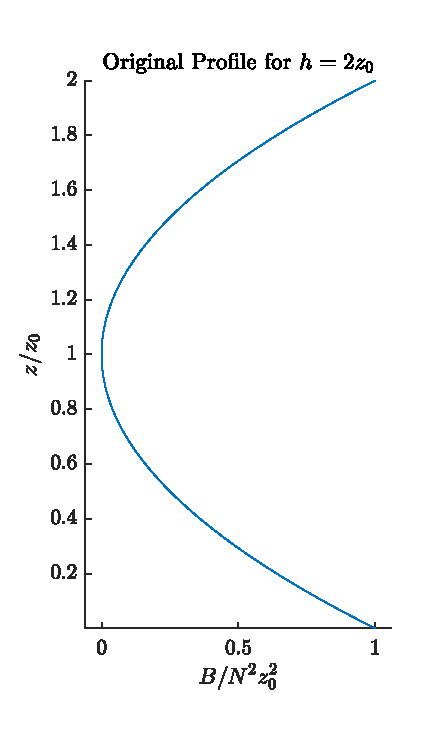
\includegraphics[scale=1]{Fig/heq2z0_org}\;\;
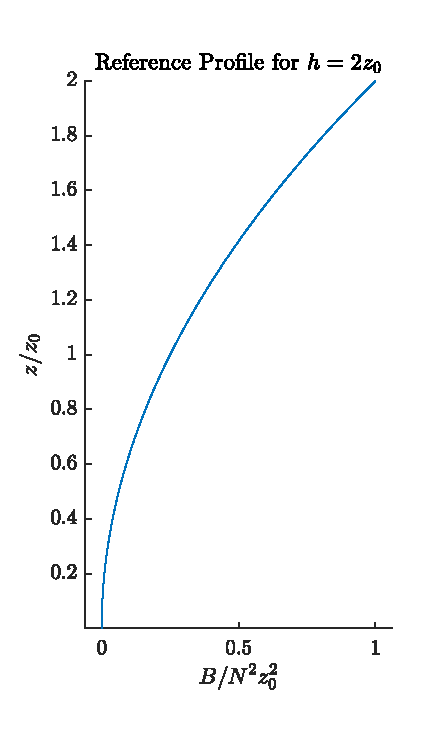
\includegraphics[scale=1]{Fig/heq2z0}
\end{center}
Then we can calculate the reference internal energy:
\begin{align*}
I_\text{ref} = \frac{N^2}{4}\int^{2z_0}_0 (z_0-z)z^2\;\de z = -\frac{N^2 z_0^4}{3}.
\end{align*}
Compare to the internal energy of the original state:
\begin{align*}
I_0 = {N^2}\int^{2z_0}_0 (z_0-z)^3\;\de z = 0.
\end{align*}
Thus the available potential energy is 
\begin{align*}
\APE = I_0-I_\text{ref} = \frac{N^2 z_0^4}{3}.
\end{align*}

For general $h$, the reference profile is a piece-wise quadratic function. Pieced together by all or parts of the reference profile above and the original profiles. We show what they look like. For $h>2z_0$:
\begin{center}
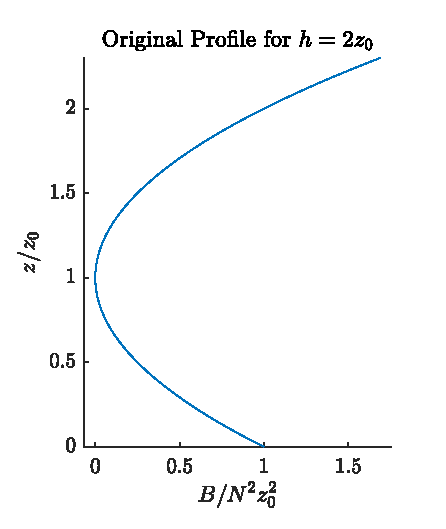
\includegraphics[scale=1]{Fig/hgg2z0_org}\;\;
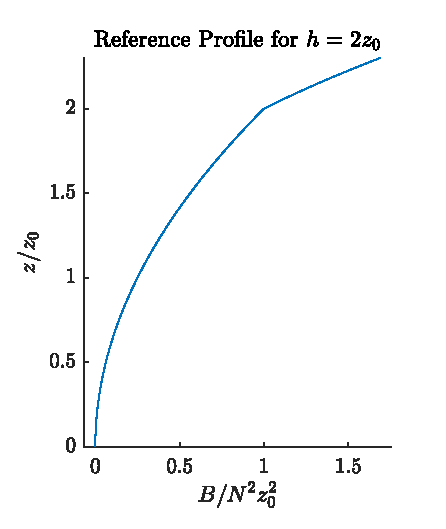
\includegraphics[scale=1]{Fig/hgg2z0}
\end{center}
It is made up of all of the reference profile for $h = 2z_0$ case at the bottom then the $2z_0<z<h$ part of the original profile above. The APE for this case is the same as the $h = 2z_0$ case:
\begin{align*}
\APE = \frac{N^2 z_0^4}{3}.
\end{align*}
For $h<2z_0$:
\begin{center}
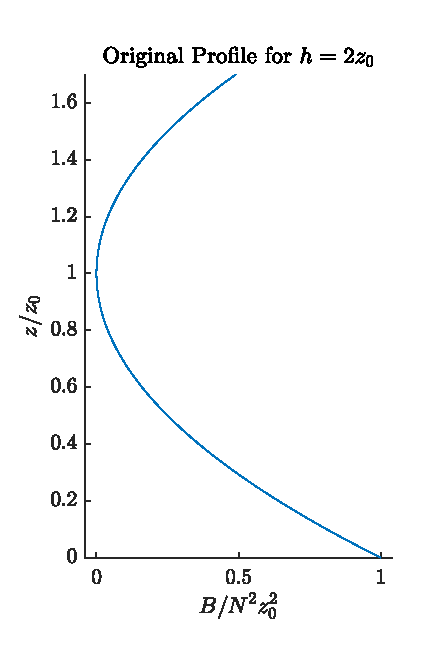
\includegraphics[scale=1]{Fig/hll2z0_org}\;\;
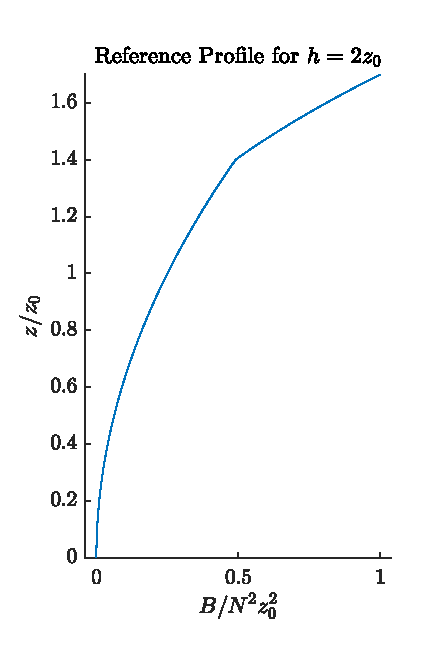
\includegraphics[scale=1]{Fig/hll2z0}
\end{center}
It is made up of the $2-h<z<h$ of the reference profile for $h = 2z_0$ case at the bottom then above that is the $0<z<2-h$ part of the original profile after a $z\to h-z$ change of variable. Given these profiles, we can calculate the APE via integration on each intervals.


\printbibliography[heading=bibintoc,title={Reference}]

\end{document}






